% Created 2016-01-27 Wed 17:27
\documentclass[11pt]{article}
\usepackage[utf8]{inputenc}
\usepackage[T1]{fontenc}
\usepackage{fixltx2e}
\usepackage{graphicx}
\usepackage{grffile}
\usepackage{longtable}
\usepackage{wrapfig}
\usepackage{rotating}
\usepackage[normalem]{ulem}
\usepackage{amsmath}
\usepackage{textcomp}
\usepackage{amssymb}
\usepackage{capt-of}
\usepackage{hyperref}
\author{B.\ Ravel, M.\ Newville, J.J.\ Kas, J.J.\ Rehr}
\date{2016-01-27}
\title{Supplemental material: The effect of self-consistent potentials on EXAFS analysis}
\hypersetup{
 pdfauthor={B.\ Ravel, M.\ Newville, J.J.\ Kas, J.J.\ Rehr},
 pdftitle={Supplemental material: The effect of self-consistent potentials on EXAFS analysis},
 pdfkeywords={},
 pdfsubject={},
 pdfcreator={Emacs 24.4.1 (Org mode 8.3.1)}, 
 pdflang={English},
 colorlinks=true,
 urlcolor=blue}

\usepackage{fullpage}
\setlength{\parindent}{0pt}
\setlength{\parskip}{2ex plus 1ex minus 1ex}

\usepackage{fancyhdr}
\pagestyle{fancy}
% \lhead{}
% \chead{}
% \rhead{\fancyplain{}{\leftmark}}
% \lfoot{}
% \cfoot{}
% \rfoot{\thepage}
\fancyhf{}
\fancyhead[L]{Self-consistency and EXAFS analysis} % predefined ()
\fancyhead[R]{\leftmark} % 1. sectionname
\fancyfoot[L]{Ravel, Newville, Kas, Rehr}
\fancyfoot[R]{\nouppercase{\thepage}}
\fancypagestyle{plain}{%
  \fancyhf{}%
  \renewcommand{\headrulewidth}{0pt}%
}
\renewcommand{\headrulewidth}{1pt}%
\renewcommand{\footrulewidth}{0pt}
\renewcommand{\headsep}{35pt}

\usepackage{titlesec}
\newcommand{\sectionbreak}{\clearpage}
\graphicspath{{/home/bruce/TeX/writing/Papers/feff85exafs/mue/}{/home/bruce/git/SCFtests/}}

\usepackage{highlight}

\begin{document}

\maketitle
\tableofcontents


\section{Background}
\label{sec:orgheadline1}


Because \textsc{feff9} is not freely available and redistributable, it
is hard to make use of it in the manner of this
exercise. Consequently, the forms of \textsc{feff} used here are the two
redistributable versions, (1) the \textsc{feff6} that comes with
\href{https://github.com/newville/ifeffit}{\textsc{ifeffit}} and (2)
\href{https://github.com/xraypy/feff85exafs}{\textsc{feff85exafs}}.

This work is about \emph{EXAFS} analysis, not XANES calculations or
calculations of other spectroscopies. Obviously, any calculation of a
spectroscopy for which the photoelectron has low kinetic energy will
be extremely sensitive to the details of the potential surface.
Self-consistency and charge transfer are
\href{http://dx.doi.org/10.1103/PhysRevB.58.7565}{unambiguously
  important} for such calculations. The question here is about the
impact on the analysis of the EXAFS spectrum.

\highlight[yellow]{SCP = Self-consistent potentials}

Here are the conditions of the tests:

\begin{enumerate}
\item All XAS data were processed sensibly in
  \href{http://bruceravel.github.io/demeter/}{\textsc{athena}} with $E_0$
  chosen to be the first peak of the first derivative in
  $\mu$(E). That may not be the best choice of $E_0$ in all cases, but it
  is the obvious first choice and the likeliest choice to be made by a
  novice user of the software.

\item All EXAFS data were Fourier transformed starting at
  3\,{\AA}$^{-1}$ and ending at a reasonable place where the signal
  was still much bigger than the noise. The choice of 3\,{\AA}$^{-1}$
  as the starting point was deliberate.  The
  \href{http://dx.doi.org/10.1103/PhysRevB.47.14126}{\textsc{autobk}
    algorithm} (and, indeed, all other algorithms) is often unreliable
  below about 3\,{\AA}$^{-1}$ due to the fact that the $\mu$(E) is
  changing very quickly in that region.  Thus the data above
  3\,{\AA}$^{-1}$ are likely to be reliably free of systematic error
  due to the details of the background removal.

\item All the materials considered have well-known structures. For
  these tests, we want to avoid the situation where error in a fitting
  model could be attributed to incomplete prior knowledge about the
  structure. That is, we want to isolate the details of the fitting
  model from the details of the theoretical calculation.

\item The first three examples are dense, crystalline solids for which
  one expects self-consistency to contribute rather little to the
  analysis.  The remaining materials all contribute interesting
  features for which self-consistency and charge transfer might play a
  role.

\item In the plots, the ranges of the Fourier transform and of the fit
  are indicated by vertical black lines.

\item Each material is fitted using theory from the version of
  \textsc{feff6} that is distributed with
  \href{https://github.com/newville/ifeffit}{the \textsc{ifeffit}
    package}, from
  \href{https://github.com/xraypy/feff85exafs}{\textsc{feff85exafs}}
  with self-consistency turned off, and from with
  \href{https://github.com/xraypy/feff85exafs}{\textsc{feff85exafs}}
  with self-consistency. In each case, the default self-energy model
  (Hedin-Lundqvist) was used.

\item For each material that is not a molecule, the analysis is done
  with a sequence of self-consistency radii. This is done to test the
  importance of the consideration of that parameter on the analysis.
  In the case of hydrated uranyl hydrate, this is a molecule, but the
  \textsc{feff} calculation is made on a crystalline analogue to the
  molecule.  The effect of self-consistency radius is tested in that
  case.

\item Where appropriate (bromoadamantane, for example), the
  \href{http://leonardo.phys.washington.edu/feff/wiki/static/s/c/f/SCF_1ebb.html}{\texttt{lfms}
    parameter of the \texttt{SCF} card} is set to 1.

\item The uranyl calculation was a bit challenging with
  \href{https://github.com/xraypy/feff85exafs}{\textsc{feff85exafs}}. To
  get the program to run to completion, it was necessary to set
  \href{http://leonardo.phys.washington.edu/feff/wiki/static/f/o/l/FOLP_93fc.html}{the
    \texttt{FOLP} parameter} to 0.9 for each unique potential. Given that the
  quality of the fit was much the same as for using \textsc{feff6},
  this was not examined further.  Still, this merits further attention
  for this material.

% \item I was interested to know if the effect of \texttt{SCF} on EXAFS fitting
%   was different for a first shell fit as compared to a more extensive
%   fitting model.  So fits were generated for the first shells only of
%   all materials except for uranyl hydrate for which the axial and
%   equatorial scatterers cannot be isolated. Also, Matt tells me that,
%   years ago, he and John looked at some \textsc{feff6/Feff8}
%   comparisons, but only for first shell fits.  These first shell fits
%   are intended for comparison to that older work.  (The results of the
%   first shell fits are included in the repository, but not on this
%   page as they do not tell a different story from the more complete
%   fits presented here.)

\item All fits were performed with a tool set written by B.\ Ravel and
  included here in this repository using the XAS analysis capabilities
  of \href{https://github.com/xraypy/xraylarch/}{\textsc{larch}}.

\item All uncertainties are 1$\sigma$ error bars determined from the
  diagonal elements of the covariance matrix evaluated during the
  Levenberg-Marquardt minimizations.  \highlight[yellow]{Say more here about
    precision of numbers in tables!}

\item The plots shown below for each material were generated
  automatically by the tool set.  You will notice that they appear to
  be highly repetitive.  For each material it is the case that the
  fits using the different theoretical models are nearly
  indistinguishable by eye.  The full complement of fits are shown for
  the sake of completeness.  Each plot is the actual plot made using
  the actual fit to the different theory models.

\item The very astute \textsc{feff} user might point out that the path
  indexing is not guaranteed to be consistent across versions.  That
  is, a small MS path may barely exceed the heap criterion in one
  version of \textsc{feff}, but not in another.  That would change the
  indexing for all paths with longer half-path-lengths, thus
  confounding the use of single \textsc{larch} fitting script with the
  different version of the theory.  To avoid this problem, the
  pathfinder in \textsc{feff6} was run, generating
  \href{http://leonardo.phys.washington.edu/feff/wiki/static/f/e/f/FEFF_Program_control_1397.html}{a
    \texttt{paths.dat} file}.  This \texttt{paths.dat} was then copied
  into the folders where the various
  \href{https://github.com/xraypy/feff85exafs}{\textsc{feff85exafs}}
  calculations were run.  The pathfinder was then skipped in each of
  the \textsc{feff8} runs.  This guaranteed that each theory
  calculation generated the same list of \texttt{feffNNNN.dat} files
  with the same indexing.

% \item For each material, a table of charge transfer and threshold
%   energies is presented. This is information gleaned from
%   \textsc{feff8}'s screen messages and \textsc{feff6}'s standard
%   header. The charge transfer values are the final charge transferred
%   for each unique potential as reported in the final round of the
%   self-consistency loop. The threshold energy $\mu$ is reported for
%   each self-consistency radius as well as for \textsc{feff8} without
%   self-consistency and for \textsc{feff6}. This table is included ion
%   hopes that it will help make sense of the fitted values for $E_0$.
\end{enumerate}

%\rule{\linewidth}{0.5pt}


\section{Copper}
\label{sec:orgheadline7}

The sample is the canonical copper foil spectrum of
\href{https://github.com/XraySpectroscopy/XAS-Data-Interchange/issues/29}{Newville,
  PhD thesis fame}. The fitting model is very simple. There is an
$S_0^2$ parameter (\texttt{amp}), an energy shift for all paths
(\texttt{enot}), and a volumetric lattice expansion coefficient
(\texttt{alpha}). The $\sigma^2$ values for all paths were computed
using the correlated Debye model and a temperature of 10K, except for
the first shell, which has its own $\sigma^2$ variable (\texttt{ss1}).

The fit included 4 coordination shells, which includes several co-linear
multiple scattering paths of the same distance as the fourth shell
single scattering path.

\texttt{amp} and \texttt{alpha} are unitless. \texttt{enot} is eV,
\texttt{ss1} is {\AA}$^2$, and \texttt{thetad} is K.

\begin{figure}[h]
  \centering
  \includegraphics[width=.65\linewidth]{copper.pdf} 
  \caption{$\mu(E)$ data for copper metal, showing the background
    removal spline and the normalization polynomials.}
  \label{fig:copper-data}
\end{figure}

\subsection{Best fit values}
\label{sec:orgheadline2}

\begin{center}
  \begin{tabular}{lrrrrr}
    model & alpha & amp & enot & ss1 & thetad\\
    \hline
    feff6        & -0.00074(92)  & 0.96(4) & 4.97(49) & 0.00382(33) & 253(22)\\
    noSCP        & -0.00046(90)  & 0.95(4) & 5.71(48) & 0.00400(33) & 239(19)\\
    withSCP(3)   & -0.00077(104) & 0.94(5) & 3.45(56) & 0.00402(38) & 241(22)\\
    withSCP(4)   & -0.00076(104) & 0.94(5) & 3.54(56) & 0.00402(38) & 242(22)\\
    withSCP(5)   & -0.00077(104) & 0.94(5) & 3.40(56) & 0.00402(38) & 241(22)\\
    withSCP(5.5) & -0.00077(105) & 0.94(5) & 3.41(56) & 0.00402(38) & 241(22)\\
    withSCP(6)   & -0.00076(104) & 0.94(5) & 3.46(56) & 0.00402(38) & 241(22)\\
  \end{tabular}
\end{center}

\subsection{Statistical parameters}
\label{sec:orgheadline3}

\begin{center}
  \begin{tabular}{lrrr}
    model & $\chi^2$ & reduced $\chi^2$ & R-factor\\
    \hline
    feff6        & 1444 & 54.4 & 0.0145\\
    noSCP        & 1414 & 53.2 & 0.0142\\
    withSCP(3)   & 1821 & 68.6 & 0.0182\\
    withSCP(4)   & 1814 & 68.3 & 0.0182\\
    withSCP(5)   & 1817 & 68.4 & 0.0182\\
    withSCP(5.5) & 1824 & 68.7 & 0.0183\\
    withSCP(6)   & 1819 & 68.5 & 0.0182\\
  \end{tabular}
\end{center}

% \subsection{Charge transfer and threshold energy}
% \label{sec:orgheadline4}

% \begin{center}
% \begin{tabular}{rrrrrr}
% ip & R=3 & R=4 & R=5 & R=5.5 & R=6\\
% \hline
% 0 & -0.527 & -0.524 & -0.512 & -0.523 & -0.516\\
% 1 & 0.005 & 0.005 & 0.005 & 0.005 & 0.005\\
% $\mu$ & -8.091 & -7.964 & -8.104 & -8.124 & -8.056\\
% \end{tabular}
% \end{center}

% Starting value for $\mu$ in \textsc{feff8} = -3.820

% Value for $\mu$ in \textsc{feff6} = -5.519

\subsection{Plots of fits}
\label{sec:orgheadline5}

\begin{center}
  \begin{tabular}{cc}
    \textbf{Feff6} & \textbf{Feff8, no SCP} \\
    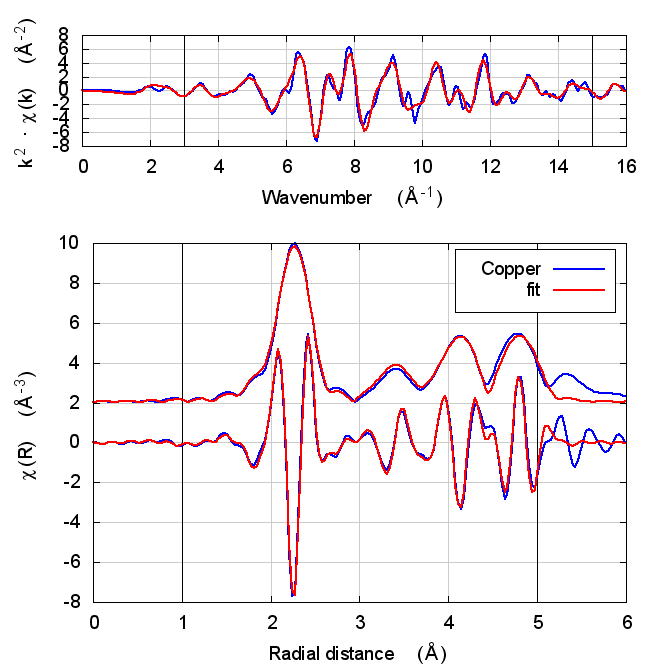
\includegraphics[width=.45\linewidth]{Copper/scf/fit_feff6.png} & 
    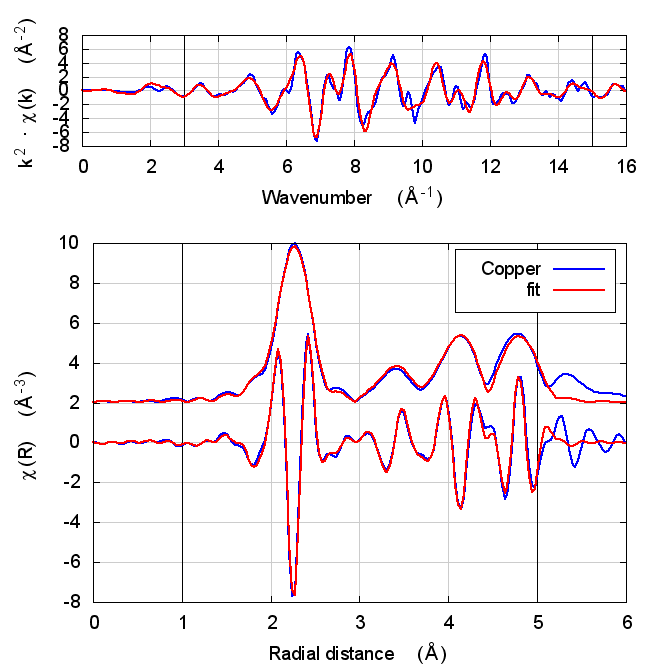
\includegraphics[width=.45\linewidth]{Copper/scf/fit_noSCF.png} \\
  \end{tabular}
\end{center}
\begin{center}
  \begin{tabular}{cc}
    \textbf{SCP, R=3} & \textbf{SCP, R=4} \\
    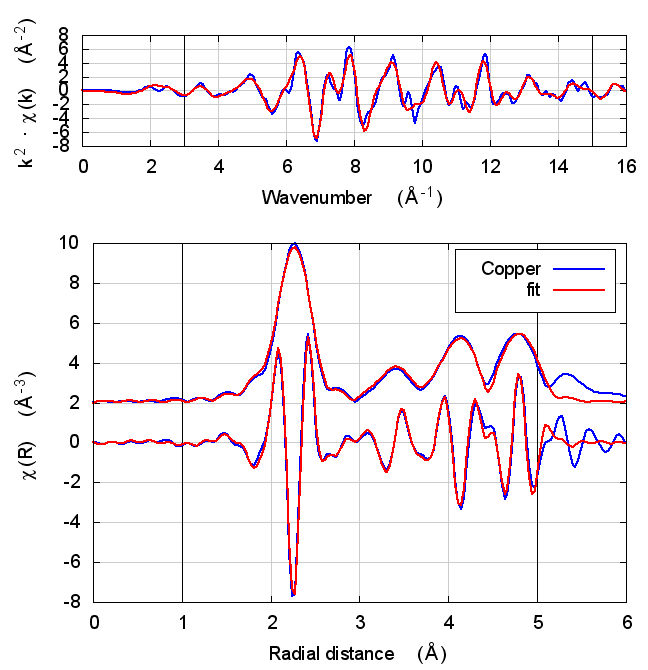
\includegraphics[width=.45\linewidth]{Copper/scf/fit_withSCF_3.png} &
    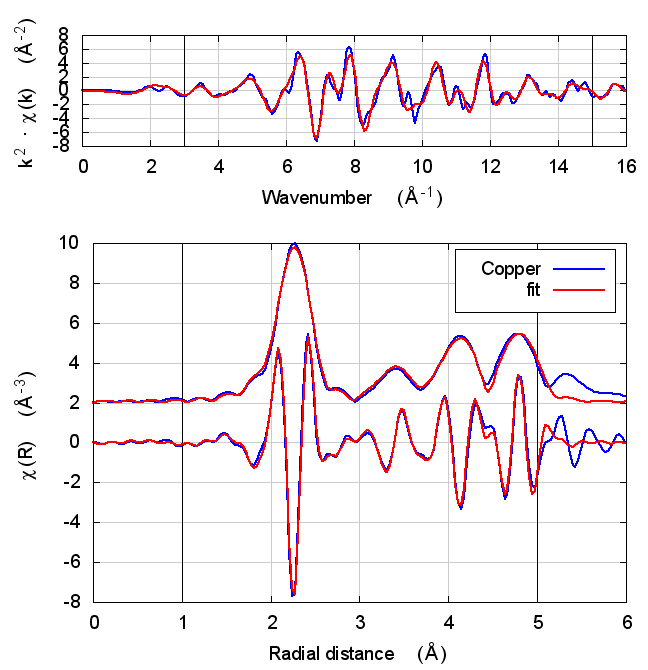
\includegraphics[width=.45\linewidth]{Copper/scf/fit_withSCF_4.png} \\
  \end{tabular}
\end{center}
\begin{center}
  \begin{tabular}{cc}
    \textbf{SCP, R=5} & \textbf{SCP, R=5.5} \\
    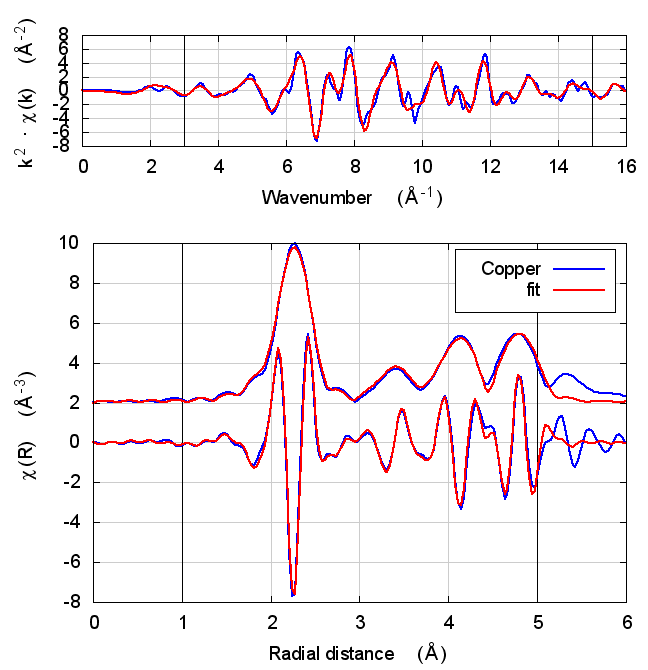
\includegraphics[width=.45\linewidth]{Copper/scf/fit_withSCF_5.png} &
    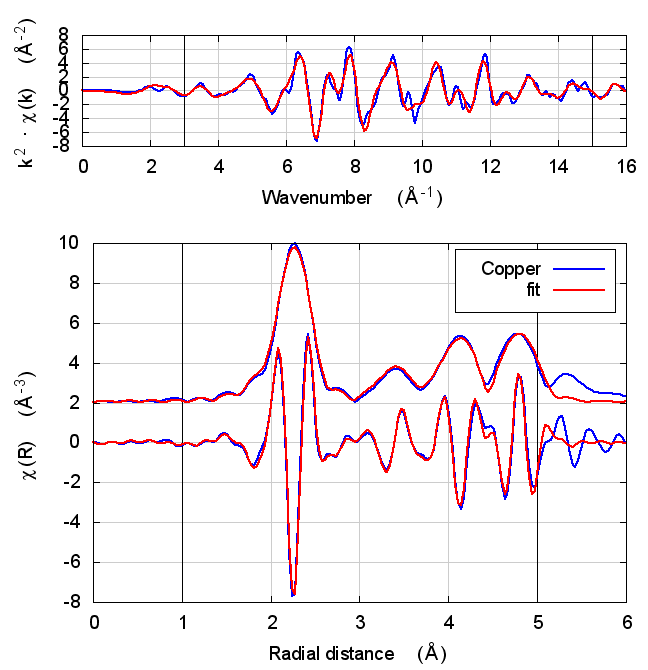
\includegraphics[width=.45\linewidth]{Copper/scf/fit_withSCF_5.5.png} \\
  \end{tabular}
\end{center}
\begin{center}
  \begin{tabular}{cc}
    \textbf{SCP, R=6} &\\
    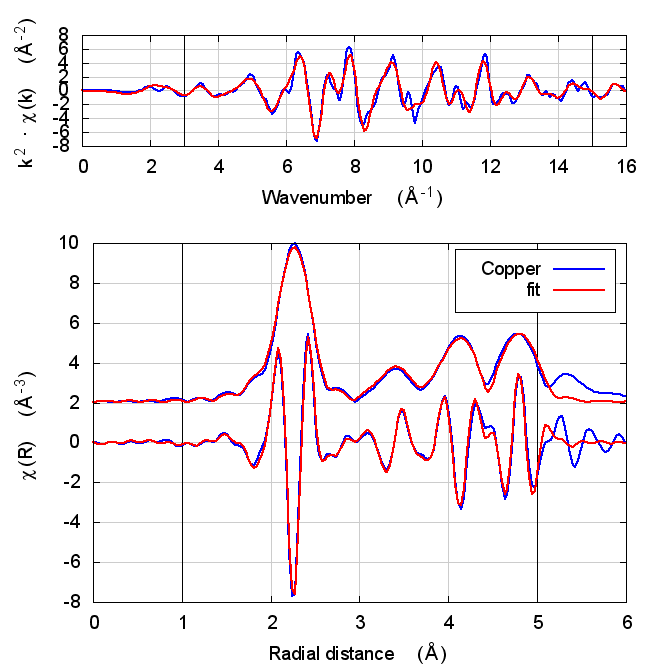
\includegraphics[width=.45\linewidth]{Copper/scf/fit_withSCF_6.png}&\\
  \end{tabular}
\end{center}


\subsection{Discussion}
\label{sec:orgheadline6}

Discussions of XAS theory historically start with copper metal.  So we
start with copper metal.

In fact, we expect copper to be a null result. There is no reason to
expect that charge transfer and self-consistency would have much effect
on a monoatomic material. That expectation is borne out.

The fitting parameters are constant well within their uncertainties
and across all theory models. The statistical parameters also do not
change much across the models. Amusingly, reduced $\chi^2$ and
R-factor are slightly smaller \emph{without} the use of
self-consistency.

%\rule{\linewidth}{0.5pt}

\section{Nickel oxide}
\label{sec:orgheadline13}

\begin{wrapfigure}{r}{0.2\textwidth}
  \begin{center}
    \includegraphics[width=0.2\textwidth]{NiO/NiO.png}
  \end{center}
  \caption{Rocksalt structure}
\end{wrapfigure}


The sample was NiO powder prepared by Dr. Neil Hyatt (University of
Sheffield) and checked by him for phase purity. The powder was mixed
with polyethylene glycol and pressed into a pellet to make a edge step
of 0.78. The data were measured at NSLS beamline X23A2 and reported in
a recent issue of Journal of Synchrotron Radiation:
\href{http://dx.doi.org/10.1107/S1600577515013521}{DOI:
  10.1107/S1600577515013521}. The simple fitting model to this rock
salt structure included a $S_0^2$ parameter (\texttt{amp}), an energy
shift (\texttt{enot}), and a volumetric lattice expansion coefficient
(\texttt{alpha}).

The fit included 4 coordination shells, 2 with O and 2 with Ni. There
are several co-linear multiple scattering paths at the same distance
as the fourth shell Ni scatterer. Each shell has its own $\sigma^2$
parameter (\texttt{sso}, \texttt{ssni}, \texttt{sso2}, and
\texttt{ssni2}, respectively.).

\texttt{amp} and \texttt{alpha} are unitless. \texttt{enot} is
eV. \texttt{sso}, \texttt{ssni}, \texttt{sso2}, and \texttt{ssni2} are
{\AA}$^2$.

\begin{figure}[h]
  \centering
  \includegraphics[width=.65\linewidth]{NiO.pdf}
  \caption{$\mu(E)$ data for NiO, showing the background
    removal spline and the normalization polynomials.}
  \label{fig:nio-data}
\end{figure}

\subsection{Best fit values}
\label{sec:orgheadline8}

\begin{center}
  \footnotesize
  \begin{tabular}{lrrrrrrr}
    model & alpha & amp & enot & ssni & ssni2 & sso & sso2\\
    \hline
    feff6        & 0.00062(146)  & 0.71(5) & -1.22(54) & 0.00546(56) & 0.00714(95) & 0.00437(120) & 0.04205(3218)\\
    noSCP        & 0.00050(152)  & 0.68(5) & 2.49(56)  & 0.00534(58) & 0.00715(101)& 0.00468(131) & 0.03946(2918)\\
    withSCP(2.5) & -0.00021(148) & 0.71(4) & -7.34(54) & 0.00554(56) & 0.00726(97) & 0.00468(123) & 0.03146(2038)\\
    withSCP(3)   & -0.00073(145) & 0.71(4) & -7.95(53) & 0.00555(55) & 0.00715(95) & 0.00456(119) & 0.03368(2237)\\
    withSCP(3.7) & -0.00068(145) & 0.71(4) & -7.94(53) & 0.00555(55) & 0.00716(95) & 0.00457(119) & 0.03344(2213)\\
    withSCP(4.2) & -0.00010(149) & 0.71(4) & -7.29(55) & 0.00554(56) & 0.00727(98) & 0.00470(124) & 0.03099(1996)\\
    withSCP(4.7) & -0.00023(148) & 0.71(4) & -7.31(54) & 0.00554(56) & 0.00725(97) & 0.00466(123) & 0.03167(2060)\\
  \end{tabular}
\end{center}

\subsection{Statistical parameters}
\label{sec:orgheadline9}

\begin{center}
  \begin{tabular}{lrrr}
    model & $\chi^2$ & reduced $\chi^2$ & R-factor\\
    \hline
    feff6        & 27430 & 1347 & 0.0215\\
    noSCP        & 29861 & 1467 & 0.0234\\
    withSCP(2.5) & 28069 & 1379 & 0.0220\\
    withSCP(3)   & 26876 & 1320 & 0.0211\\
    withSCP(3.7) & 26950 & 1324 & 0.0211\\
    withSCP(4.2) & 28301 & 1390 & 0.0222\\
    withSCP(4.7) & 28050 & 1378 & 0.0220\\
  \end{tabular}
\end{center}

% \subsection{Charge transfer and threshold energy}
% \label{sec:orgheadline10}

% \begin{center}
% \begin{tabular}{rrrrrr}
% ip & R=2.5 & R=3 & R=3.7 & R=4.2 & R=4.7\\
% \hline
% 0 & 0.084 & 0.150 & 0.145 & 0.092 & 0.080\\
% 1 & 0.090 & 0.177 & 0.171 & 0.092 & 0.104\\
% 2 & -0.091 & -0.179 & -0.172 & -0.093 & -0.105\\
% $\mu$ & -12.012 & -12.768 & -12.749 & -11.952 & -11.973\\
% \end{tabular}
% \end{center}

% Starting value for $\mu$ in \textsc{feff8} = -3.100

% Value for $\mu$ in \textsc{feff6} = -3.478

\subsection{Plots of fits}
\label{sec:orgheadline11}

\begin{center}
  \begin{tabular}{cc}
    \textbf{Feff6} & \textbf{Feff8, no SCP} \\
    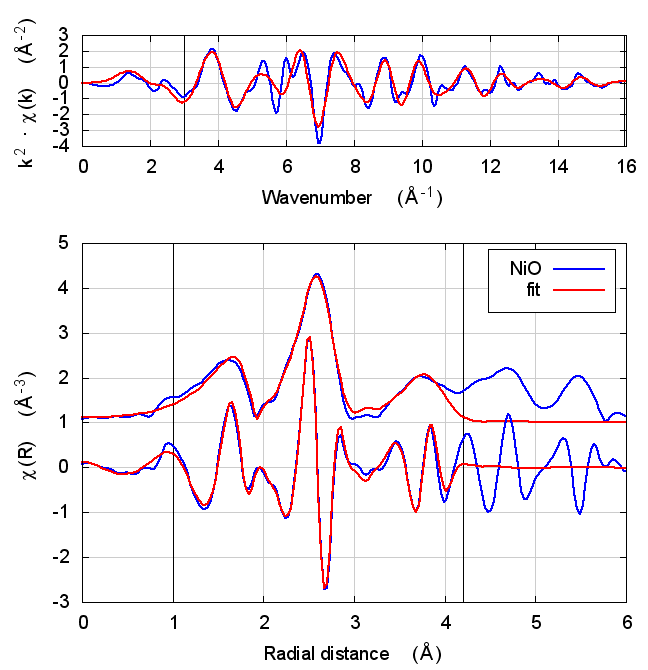
\includegraphics[width=.45\linewidth]{NiO/scf/fit_feff6.png} & 
    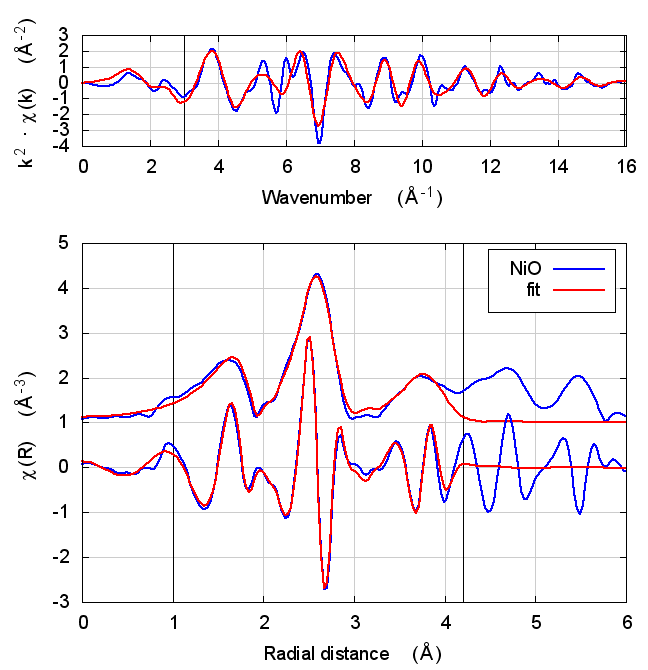
\includegraphics[width=.45\linewidth]{NiO/scf/fit_noSCF.png} \\
  \end{tabular}
\end{center}
\begin{center}
  \begin{tabular}{cc}
    \textbf{SCP, R=2.5} & \textbf{SCP, R=3} \\
    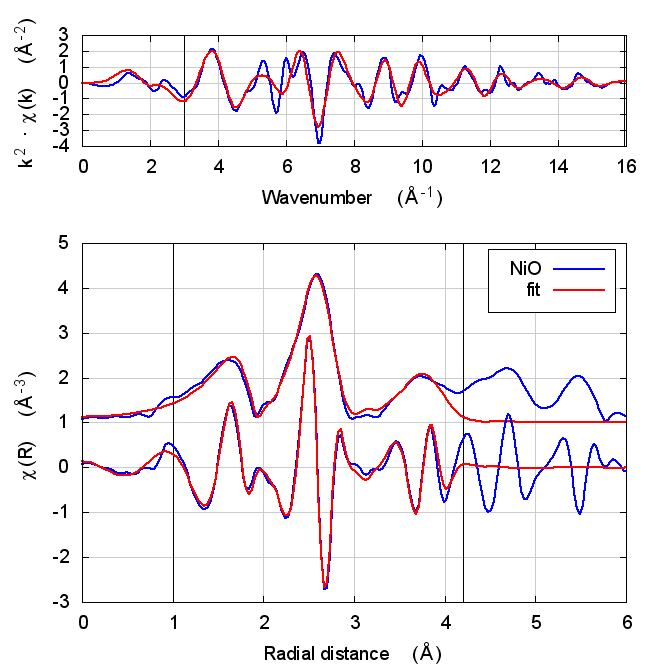
\includegraphics[width=.45\linewidth]{NiO/scf/fit_withSCF_2.5.png} & 
    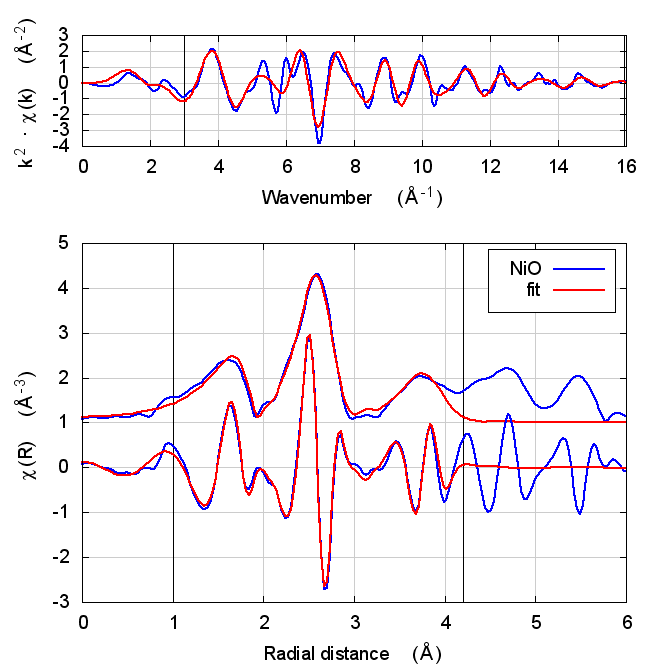
\includegraphics[width=.45\linewidth]{NiO/scf/fit_withSCF_3.png} \\
  \end{tabular}
\end{center}
\begin{center}
  \begin{tabular}{cc}
    \textbf{SCP, R=3.7} & \textbf{SCP, R=4.2} \\
    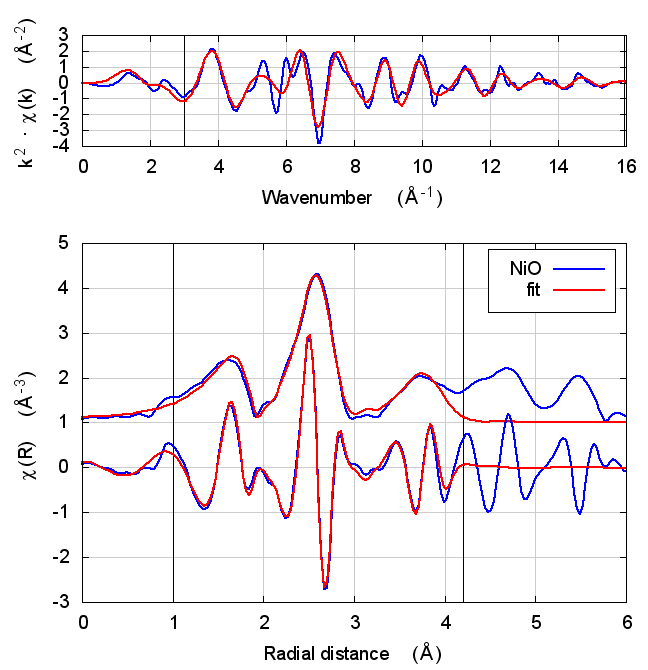
\includegraphics[width=.45\linewidth]{NiO/scf/fit_withSCF_3.7.png} & 
    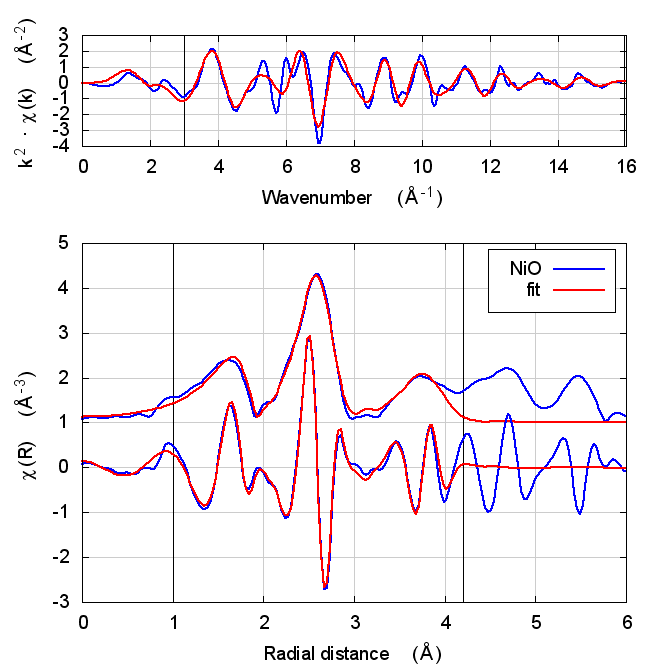
\includegraphics[width=.45\linewidth]{NiO/scf/fit_withSCF_4.2.png} \\
  \end{tabular}
\end{center}
\begin{center}
  \begin{tabular}{cc}
    \textbf{SCP, R=4.7}&\\
    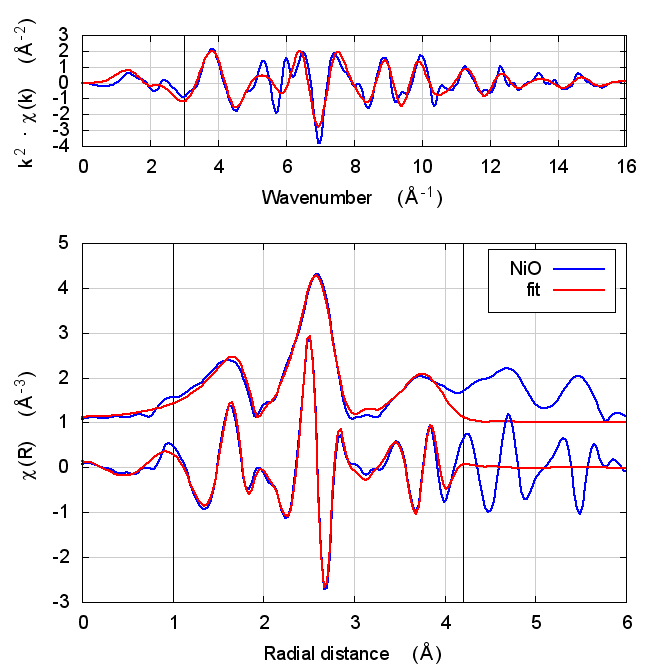
\includegraphics[width=.45\linewidth]{NiO/scf/fit_withSCF_4.7.png}&\\
  \end{tabular}
\end{center}

\subsection{Discussion}
\label{sec:orgheadline12}

NiO was chosen as the second example because it constitutes the smallest
added complexity compared to copper. NiO is a rock salt structure, so it
is highly ordered and the local configuration around the Ni atom is very
well known. With an oxygen ligand, there should be some charge transfer.

With the exception of the $E_0$ parameter, all of the parameters are
constant well within their error bars. The statistical parameters are
unchanged from model to model.

This is the first example of dependence of the $E_0$ parameter on
theoretical model. The ultimate value of \textsc{feff}'s threshold
energy depends on the model. The starting condition is not the same in
\textsc{feff6} as in \textsc{feff8} without self-consistency. This is
seen by the 3.3 eV shift in fitted $E_0$ value. Furthermore, the
threshold changes as charge is transferred and self-consistency is
reached. This results in a -6 eV shift relative to \textsc{feff6}.

A standard explanation of the $E_0$ fitting parameter is that it is the
parameter that lines up the zero of wavenumber in the data with the
zero of wavenumber in the theory. As such, it is hard to say that one
of these $E_0$ results is ``better'' than the others.

One might hope that improvements in theory would lead to a fitted $E_0$
parameter of 0 when the edge is chosen at the inflection point of the
rising edge of the XAS data.  See the manuscript for more discussion
on this.

%\rule{\linewidth}{0.5pt}
%\pagebreak

\section{Pyrite (iron sulfide)}
\label{sec:orgheadline19}

\begin{wrapfigure}{r}{0.3\textwidth}
  \begin{center}
    \includegraphics[width=0.3\textwidth]{FeS2/FeS2.png}
  \end{center}
  \caption{Pyrite structure}
\end{wrapfigure}


This is a
\href{https://github.com/bruceravel/XAS-Education/tree/master/Examples/FeS2}{standard
  teaching example}. It's good for teaching as it is fairly simple --
it's cubic -- but it has a bit of structure and two kinds of
scatterers.  The data are taken from
\href{http://cars.uchicago.edu/~newville/ModelLib/search.html}{an
  online collection of reference spectra}.

The model includes a $S_0^2$ parameter (\texttt{amp}), an energy shift
(\texttt{enot}), and a volumetric lattice expansion coefficient
(\texttt{alpha}). The first and second shell S scatterers each get a
$\sigma^2$ parameter (\texttt{ss} and \texttt{ss2}). The third shell
of S atoms only contains 2 scatterers. In practice, floating its
$\sigma^2$ parameter independently does not yield a statistical
improvement to the fit, so the \texttt{ss2} parameter is used for the
third shell $\sigma^2$.  Finally a $\sigma^2$ parameter is floated for
the Fe shell.

The fitting model includes a variety of multiple scattering paths,
including a triangle between the first shell S and the fourth shell
Fe, and four paths that bounce around among first shell S atoms.

\texttt{amp} and \texttt{alpha} are unitless. \texttt{enot} is
eV. \texttt{ss}, \texttt{ss2}, and \texttt{ssfe} are {\AA}$^2$.

\begin{figure}[h]
  \centering
  \includegraphics[width=.65\linewidth]{FeS2.pdf} 
  \caption{$\mu(E)$ data for FeS$_2$, showing the background
    removal spline and the normalization polynomials.}
  \label{fig:fes2-data}
\end{figure}


\subsection{Best fit values}
\label{sec:orgheadline14}

\begin{center}
  \footnotesize
  \begin{tabular}{lrrrrrr}
    model & alpha & amp & enot & ss & ss2 & ssfe\\
    \hline
    feff6        & 0.00092(126) & 0.69(2) &  2.77(42) & 0.00296(41) & 0.00366(106) & 0.00484(50)\\
    noSCP        & 0.00183(171) & 0.65(3) &  7.01(57) & 0.00294(57) & 0.00386(151) & 0.00471(68)\\
    withSCP(3)   & 0.00219(191) & 0.68(3) & -2.01(63) & 0.00311(63) & 0.00422(172) & 0.00495(77)\\
    withSCP(3.6) & 0.00212(188) & 0.68(3) & -2.15(62) & 0.00311(62) & 0.00423(170) & 0.00495(76)\\
    withSCP(4)   & 0.00212(191) & 0.68(3) & -2.17(63) & 0.00311(63) & 0.00423(172) & 0.00494(77)\\
    withSCP(5.3) & 0.00216(194) & 0.68(4) & -1.92(64) & 0.00310(64) & 0.00421(175) & 0.00493(78)\\
    withSCP(5.5) & 0.00216(194) & 0.68(4) & -1.88(64) & 0.00310(64) & 0.00421(175) & 0.00493(78)\\
  \end{tabular}
\end{center}

\subsection{Statistical parameters}
\label{sec:orgheadline15}

\begin{center}
  \begin{tabular}{lrrr}
    model & $\chi^2$ & reduced $\chi^2$ & R-factor\\
    \hline
    feff6        & 2052 & 146.4 & 0.0064\\
    noSCP        & 3783 & 269.9 & 0.0119\\
    withSCP(3)   & 4639 & 331.0 & 0.0146\\
    withSCP(3.6) & 4503 & 321.3 & 0.0141\\
    withSCP(4)   & 4635 & 330.7 & 0.0145\\
    withSCP(5.3) & 4778 & 341.0 & 0.0150\\
    withSCP(5.5) & 4798 & 342.4 & 0.0151\\
  \end{tabular}
\end{center}

% \subsection{Charge transfer and threshold energy}
% \label{sec:orgheadline16}

% \begin{center}
% \begin{tabular}{rrrrrr}
% ip & R=3 & R=3.6 & R=4 & R=5.3 & R=5.5\\
% \hline
% 0 & -0.332 & -0.346 & -0.359 & -0.378 & -0.376\\
% 1 & -0.325 & -0.346 & -0.380 & -0.396 & -0.397\\
% 2 & 0.164 & 0.175 & 0.192 & 0.200 & 0.201\\
% $\mu$ & -9.464 & -9.555 & -9.671 & -9.488 & -9.465\\
% \end{tabular}
% \end{center}

% Starting value for $\mu$ in \textsc{feff8} = -0.796

% Value for $\mu$ in \textsc{feff6} = -4.308

\subsection{Plots of fits}
\label{sec:orgheadline17}

\begin{center}
  \begin{tabular}{cc}
    \textbf{Feff6} & \textbf{Feff8, no SCP} \\ 
    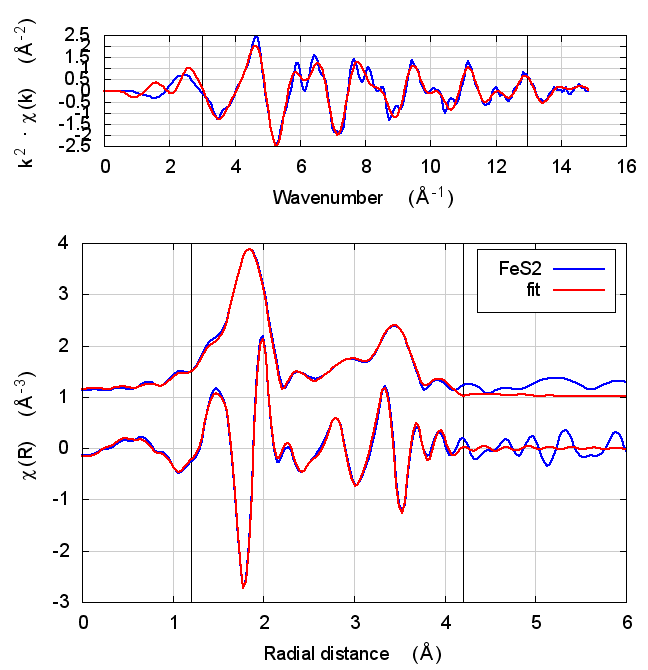
\includegraphics[width=.45\linewidth]{FeS2/scf/fit_feff6.png} & 
    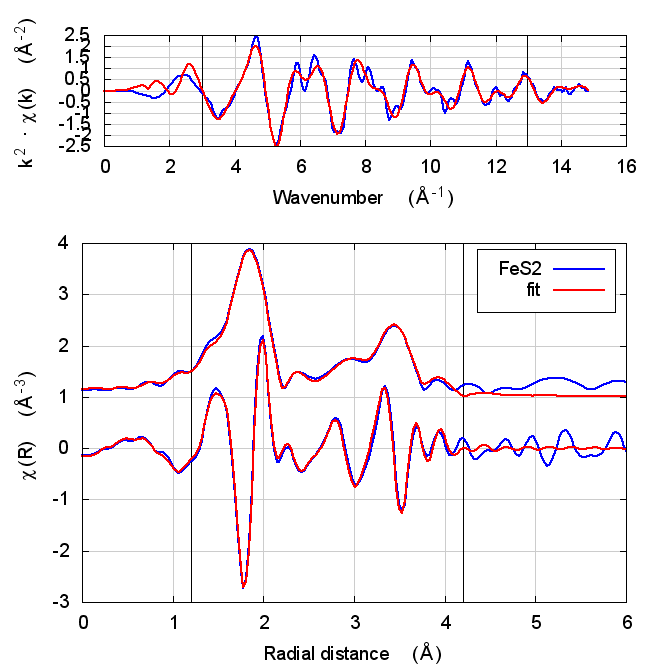
\includegraphics[width=.45\linewidth]{FeS2/scf/fit_noSCF.png} \\
  \end{tabular}
\end{center}
\begin{center}
  \begin{tabular}{cc}
    \textbf{SCP, R=3} & \textbf{SCP, R=3.6} \\ 
    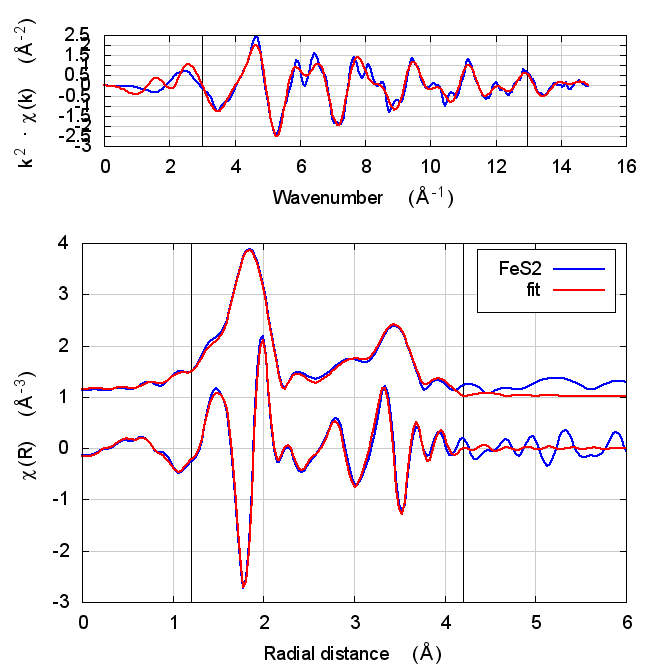
\includegraphics[width=.45\linewidth]{FeS2/scf/fit_withSCF_3.png} & 
    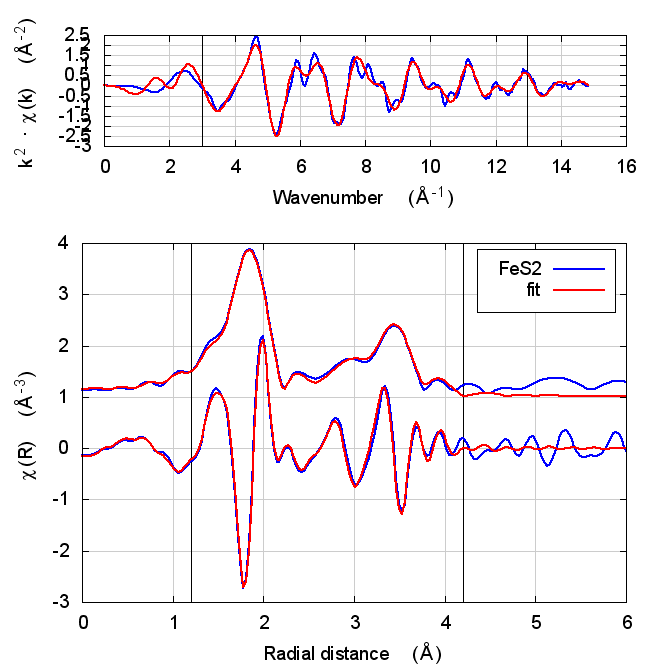
\includegraphics[width=.45\linewidth]{FeS2/scf/fit_withSCF_3.6.png} \\
  \end{tabular}
\end{center}
\begin{center}
  \begin{tabular}{cc}
    \textbf{SCP, R=4} & \textbf{SCP, R=5.3} \\
    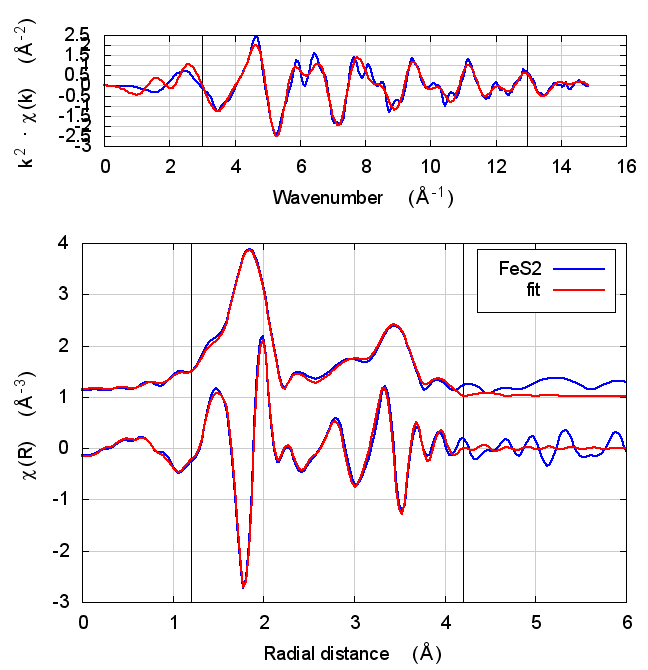
\includegraphics[width=.45\linewidth]{FeS2/scf/fit_withSCF_4.png} & 
    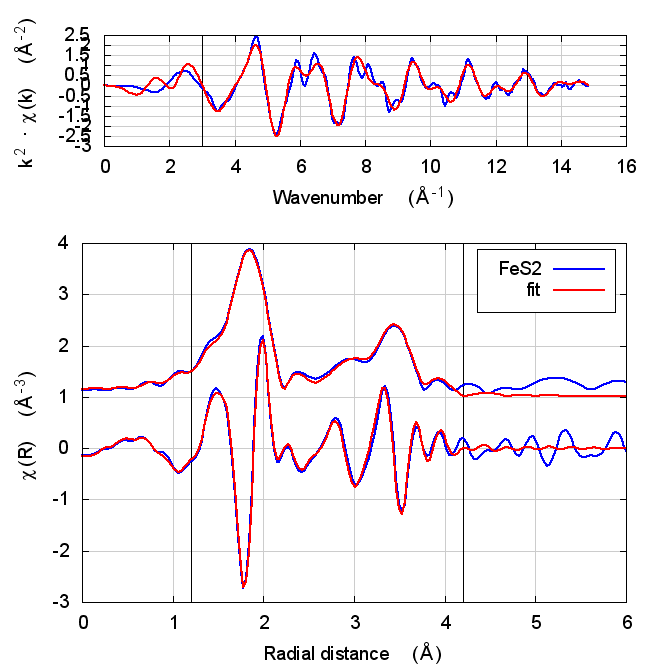
\includegraphics[width=.45\linewidth]{FeS2/scf/fit_withSCF_5.3.png} \\
  \end{tabular}
\end{center}
\begin{center}
  \begin{tabular}{cc}
    \textbf{SCP, R=5.5}&\\
    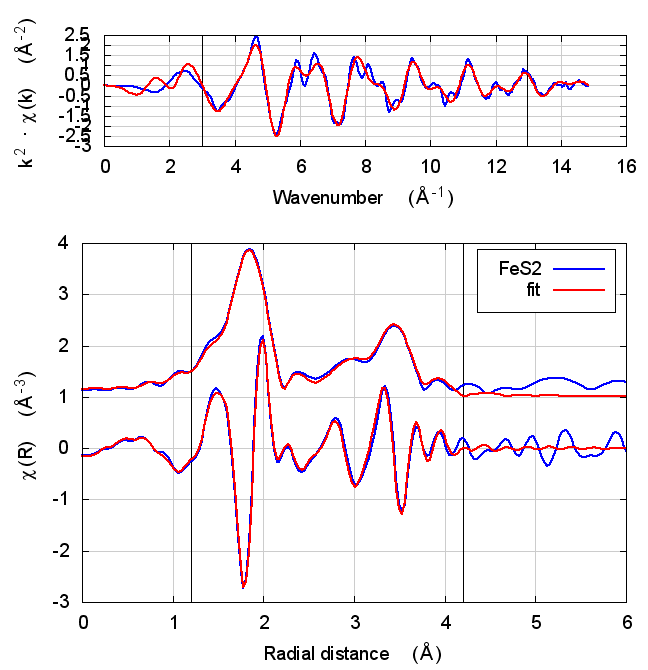
\includegraphics[width=.45\linewidth]{FeS2/scf/fit_withSCF_5.5.png}&\\
  \end{tabular}
\end{center}

\subsection{Discussion}
\label{sec:orgheadline18}

This is just slightly more complex than NiO. It is diatomic, but with
a slightly less orderly structure than NiO. Again, all parameters
except for $E_0$ are consistent within uncertainty, although the $\alpha$
parameter does show some correlation with $E_0$. All other parameters are
essentially unchanged.

The $E_0$ parameter, with self-consistency, is equally far from 0 as for
\textsc{feff6}, although with a sign change.

There are a small handful of small MS paths with half-path-lengths
within the fitting range but which are not included in this fit. This
may account for the increase in reduced $\chi^2$ and R-factor between
\textsc{feff6} and \textsc{feff8}.

%\rule{\linewidth}{0.5pt}
%\pagebreak

\section{Uraninite}
\label{sec:orgheadline25}

\begin{wrapfigure}{r}{0.3\textwidth}
  \begin{center}
    \includegraphics[width=0.3\textwidth]{UO2/UO2.png}
  \end{center}
  \caption{Uraninite}
\end{wrapfigure}


The data are the UO2 shown in Shelly's paper on \textit{Reduction of
  Uranium(VI) by Mixed Iron(II)/Iron(III) Hydroxide (Green Rust):
  Formation of UO2 Nanoparticles}:
\href{http://dx.doi.org/10.1021/es0208409}{DOI: 10.1021/es0208409}

This is an interesting test as it is an f-electron system.

The fitting model follows rather closely to what is described in that
paper, particularly the content of Table 2, although I allow $S_0^2$
to float (\texttt{amp}). Along with an energy shift (\texttt{enot}), a
$\Delta$R and $\sigma^2$ for the first shell O (\texttt{dro} and
\texttt{sso}), a $\Delta$R and $\sigma^2$ for the second shell U
(\texttt{dru} and \texttt{ssu}), and a $\Delta$R and $\sigma^2$ for
the third shell O (\texttt{dro2} and \texttt{sso2}), there is a
parameter for the number of U scatterers (\texttt{nu}).

The model includes the same 6 paths given in Table 2 of Shelly's
paper.

\texttt{amp} is unitless. \texttt{enot} is eV. \texttt{dro},
\texttt{dru}, and \texttt{dro2} are {\AA}. \texttt{sso}, \texttt{ssu},
and \texttt{sso2} are \AA$^2$.

\begin{figure}[h]
  \centering
  \includegraphics[width=.65\linewidth]{UO2.pdf} 
  \caption{$\mu(E)$ data for UO$_2$, showing the background
    removal spline and the normalization polynomials.}
  \label{fig:uo2-data}
\end{figure}


\subsection{Best fit values}
\label{sec:orgheadline20}

\begin{center}
  \footnotesize
  \begin{tabular}{lrrrrrrrrr}
    model & amp & dro & dro2 & dru & enot & nu \\
    \hline
    feff6        & 0.87(11) & -0.022(14) & -0.055(24) &  0.005(11) & 4.87(1.36) & 11.43(4.81) \\
    noSCP        & 0.84(11) & -0.023(15) & -0.024(32) &  0.001(12) & 8.15(1.46) &  9.27(4.16) \\
    withSCP(3)   & 0.84(10) & -0.026(13) & -0.013(28) & -0.002(11) & 1.63(1.29) &  9.21(3.76) \\
    withSCP(4)   & 0.84(10) & -0.026(13) & -0.013(29) & -0.003(11) & 2.08(1.30) &  9.16(3.73) \\
    withSCP(5)   & 0.84(10) & -0.026(13) & -0.012(28) & -0.003(11) & 1.72(1.29) &  9.18(3.73) \\
    withSCP(5.5) & 0.84(10) & -0.026(13) & -0.012(28) & -0.003(11) & 1.62(1.29) &  9.17(3.72) \\
    withSCP(6)   & 0.84(10) & -0.026(13) & -0.012(29) & -0.003(11) & 1.71(1.29) &  9.16(3.72) \\
  \end{tabular}

  \begin{tabular}{lrrr}
    model & sso & sso2 & ssu\\
    \hline
    feff6        & 0.00939(213) & 0.01060(440) & 0.00488(247)\\
    noSCP        & 0.00872(221) & 0.01061(618) & 0.00382(273)\\
    withSCP(3)   & 0.00894(209) & 0.00976(511) & 0.00393(250)\\
    withSCP(4)   & 0.00892(209) & 0.00972(513) & 0.00389(250)\\
    withSCP(5)   & 0.00893(208) & 0.00969(508) & 0.00391(249)\\
    withSCP(5.5) & 0.00894(208) & 0.00970(509) & 0.00391(249)\\
    withSCP(6)   & 0.00893(208) & 0.00971(510) & 0.00390(249)\\
  \end{tabular}
\end{center}

\subsection{Statistical parameters}
\label{sec:orgheadline21}

\begin{center}
  \begin{tabular}{lrrr}
    model & $\chi^2$ & reduced $\chi^2$ & R-factor\\
    \hline
    feff6        & 166.3 & 22.1 & 0.0160\\
    noSCP        & 188.4 & 25.0 & 0.0181\\
    withSCP(3)   & 169.6 & 22.5 & 0.0163\\
    withSCP(4)   & 170.0 & 22.6 & 0.0163\\
    withSCP(5)   & 169.1 & 22.4 & 0.0163\\
    withSCP(5.5) & 169.1 & 22.4 & 0.0163\\
    withSCP(6)   & 169.2 & 22.5 & 0.0163\\
  \end{tabular}
\end{center}

% \subsection{Charge transfer and threshold energy}
% \label{sec:orgheadline22}

% \begin{center}
% \begin{tabular}{rrrrrr}
% ip & R=3 & R=4 & R=5 & R=5.5 & R=6\\
% \hline
% 0 & 1.122 & 1.146 & 1.180 & 1.189 & 1.191\\
% 1 & 0.715 & 0.726 & 0.740 & 0.745 & 0.741\\
% 2 & -0.363 & -0.369 & -0.376 & -0.379 & -0.377\\
% $\mu$ & -8.541 & -8.114 & -8.522 & -8.624 & -8.542\\
% \end{tabular}
% \end{center}

% Starting value for $\mu$ in \textsc{feff8} = -0.640

% Value for $\mu$ in \textsc{feff6} = -6.058

\subsection{Plots of fits}
\label{sec:orgheadline23}

\begin{center}
  \begin{tabular}{cc}
    \textbf{Feff6} & \textbf{Feff8, no SCP} \\ 
    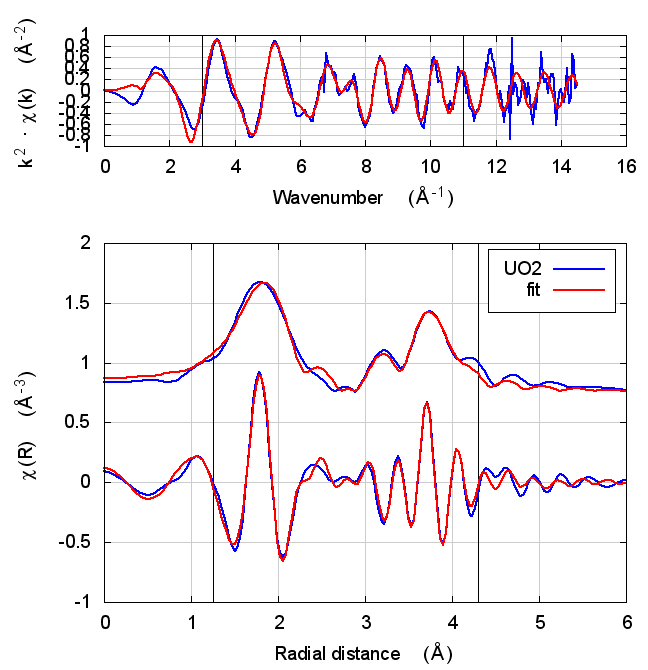
\includegraphics[width=.45\linewidth]{UO2/scf/fit_feff6.png} & 
    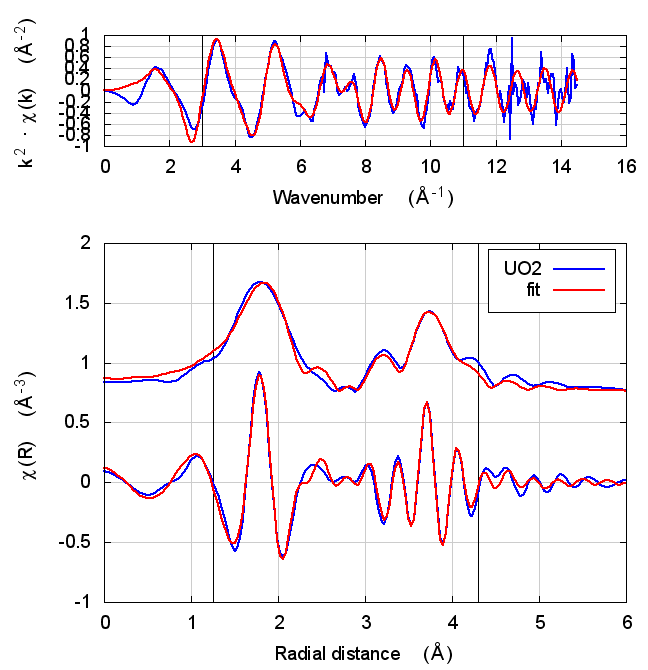
\includegraphics[width=.45\linewidth]{UO2/scf/fit_noSCF.png} \\
  \end{tabular}
\end{center}
\begin{center}
  \begin{tabular}{cc}
    \textbf{SCP, R=3} & \textbf{SCP, R=4} \\ 
    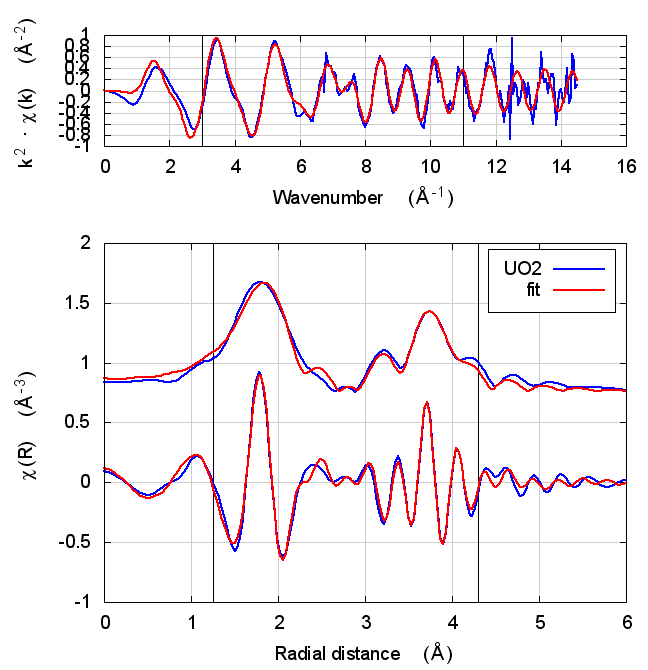
\includegraphics[width=.45\linewidth]{UO2/scf/fit_withSCF_3.png} & 
    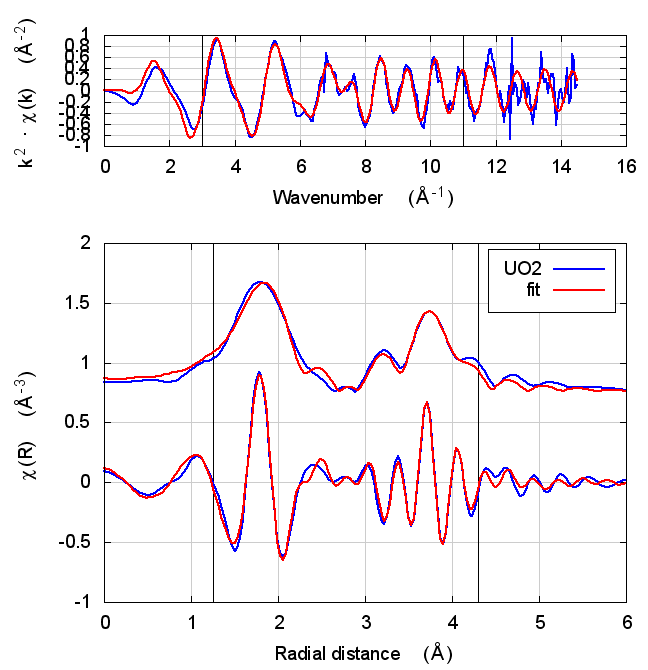
\includegraphics[width=.45\linewidth]{UO2/scf/fit_withSCF_4.png} \\
  \end{tabular}
\end{center}
\begin{center}
  \begin{tabular}{cc}
    \textbf{SCP, R=5} & \textbf{SCP, R=5.5} \\ 
    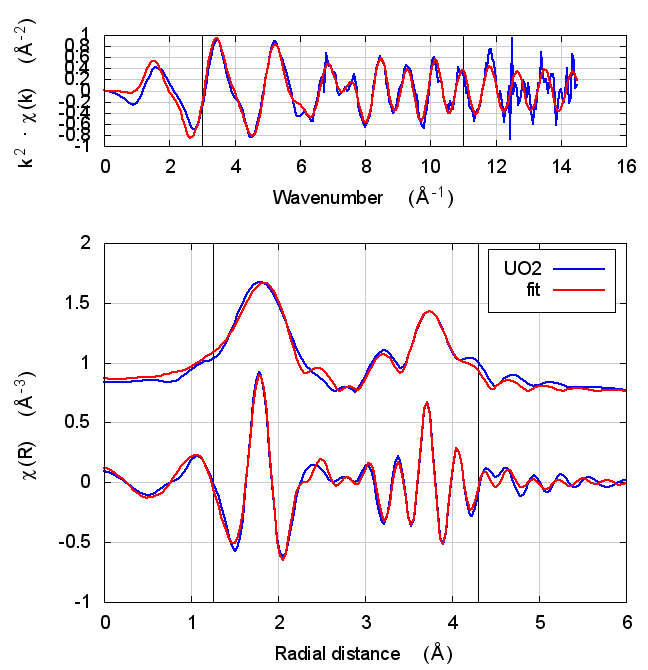
\includegraphics[width=.45\linewidth]{UO2/scf/fit_withSCF_5.png} & 
    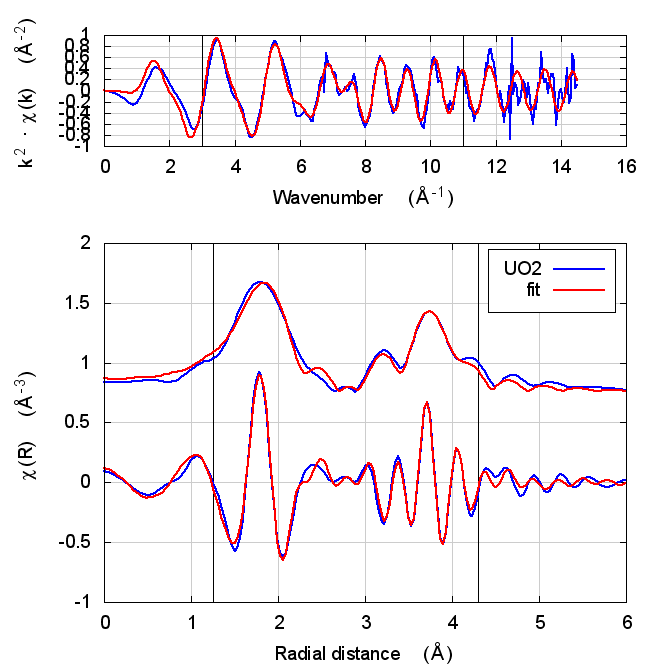
\includegraphics[width=.45\linewidth]{UO2/scf/fit_withSCF_5.5.png} \\
  \end{tabular}
\end{center}
\begin{center}
  \begin{tabular}{cc}
    \textbf{SCP, R=6}&\\
    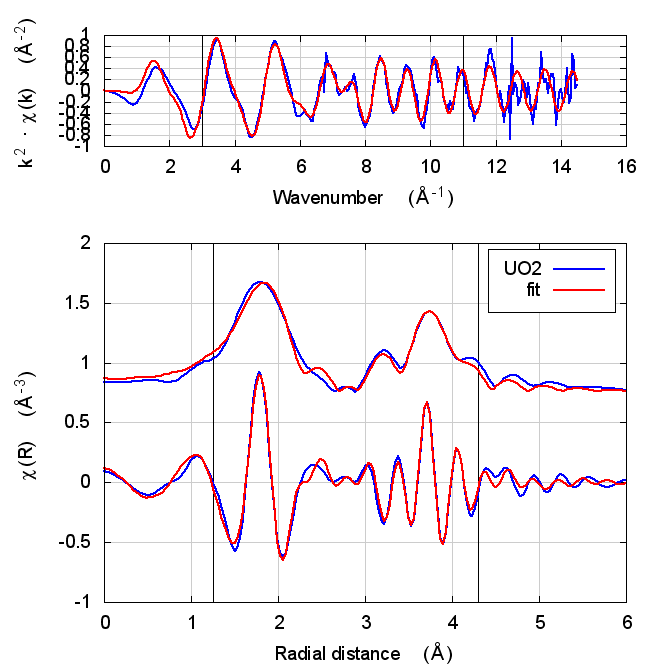
\includegraphics[width=.45\linewidth]{UO2/scf/fit_withSCF_6.png}&\\
  \end{tabular}
\end{center}

\subsection{Discussion}
\label{sec:orgheadline24}

The first thing to notice about UO2 is that the statistical parameters
of the fit are completely unchanged between theory models.

This $E_0$ parameter is the first one that behaves in the expected way --
with self-consistency and charge transfer, the fitted $E_0$ ends up
closer to 0. Perhaps this is a hint that self-consistency is important
for f-electron systems.

All of the other fitting parameters are unchanged within their
uncertainties. One parameter merits a bit more discussion. In the
paper cited above, the fitted value of \texttt{nu}, i.e. the partial
occupancy of the U atom in the second scattering shell, is used to say
something about the size of the uraninite nanoparticles generated by
the reduction process. While the fitted value of \texttt{nu} does not
change outside of its very large uncertainty, it does change
substantively. This would likely effect the interpretation of the
fitting results in the context of the reduction process.

%\rule{\linewidth}{0.5pt}
%\pagebreak

\section{Barium zirconate}
\label{sec:orgheadline31}

\begin{wrapfigure}{r}{0.2\textwidth}
  \begin{center}
    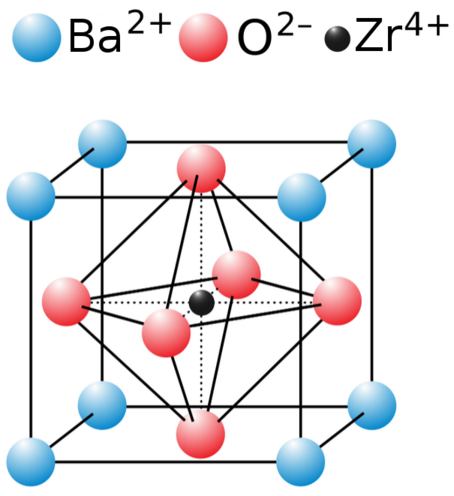
\includegraphics[width=0.2\textwidth]{BaZrO3/perovskite.png}
  \end{center}
  \caption{The perovskite structure}
\end{wrapfigure}


In a short paper on the Zr edge of BaZrO3,
\href{http://dx.doi.org/10.1016/0921-4526(94)00654-E}{DOI:
  10.1016/0921-4526(94)00654-E}, Haskel et al. proposed that
shortcomings of \textsc{feff}'s potential model could be accommodated by
floating an energy shift parameter for each scatterer species. The
concept is that doing so approximates the effect of errors in the
scattering phase shifts.

The data are the same as in that paper, although the fitting model is
slightly different. Rather than floating $\Delta$R parameters for each
shell, I used a volumetric expansion coefficient
(\texttt{alpha}). Along with $S_0^2$ (\texttt{amp}), there are energy
shifts for each scatterer (\texttt{enot}, \texttt{ezr}, and
\texttt{eba}) and $\sigma^2$ parameters for each scatterer
(\texttt{sso}, \texttt{sszr}, and \texttt{ssba}.  The fourth shell O
is included in the fit. It gets a $\sigma^2$ (\texttt{sso2}) but uses
the energy shift for the O scatterer.

BaZrO3 is a true perovskite. Zr sites in the octahedral B site. A
variety of co-linear multiple scattering paths at the distance of the
third shell Zr scatterer are included in the fit. The energy shifts are
parametrized as described in the paper.

\texttt{amp} and \texttt{alpha} are unitless. \texttt{enot}, \texttt{ezr}, and \texttt{eba} are eV. \texttt{sso},
\texttt{sszr}, \texttt{ssba}, and \texttt{sso2} are {\AA}$^2$.

\begin{figure}[h]
  \centering
  \includegraphics[width=.65\linewidth]{BaZrO3.pdf} 
  \caption{$\mu(E)$ data for the Zr edge of BaZrO$_3$, showing the
    background removal spline and the normalization polynomials.}
  \label{fig:bazro3-data}
\end{figure}


\subsection{Best fit values}
\label{sec:orgheadline26}

\begin{center}
  \footnotesize
  \begin{tabular}{lrrrrr}
    model & alpha & amp & eba & enot & ezr \\
    \hline
    feff6        & -0.00032(85) & 1.22(7) &  -9.91(57) &  -8.55(57) & -5.60(1.72) \\
    noSCP        &  0.00044(86) & 1.07(6) &  -3.90(59) &  -2.32(58) &  0.95(1.89) \\
    withSCP(3)   & -0.00007(72) & 1.13(5) & -10.77(47) & -10.52(47) & -6.68(1.58) \\
    withSCP(4)   & -0.00007(74) & 1.13(5) & -11.03(48) & -10.60(48) & -6.79(1.62) \\
    withSCP(5)   & -0.00007(73) & 1.13(5) & -11.09(48) & -10.81(48) & -7.06(1.60) \\
    withSCP(5.5) & -0.00007(73) & 1.13(5) & -10.95(48) & -10.77(48) & -7.05(1.59) \\
    withSCP(6)   & -0.00005(73) & 1.13(5) & -10.71(47) & -10.49(48) & -6.73(1.59) \\
  \end{tabular}

  \begin{tabular}{lrrrr}
    model  & ssba & sso & sso2 & sszr\\
    \hline
    feff6        & 0.00561(37) & 0.00403(70) & 0.00908(253) & 0.00413(33)\\
    noSCP        & 0.00530(38) & 0.00361(70) & 0.00791(242) & 0.00369(34)\\
    withSCP(3)   & 0.00561(32) & 0.00382(58) & 0.00855(208) & 0.00362(28)\\
    withSCP(4)   & 0.00559(33) & 0.00380(59) & 0.00850(213) & 0.00362(28)\\
    withSCP(5)   & 0.00561(33) & 0.00381(59) & 0.00850(211) & 0.00363(28)\\
    withSCP(5.5) & 0.00562(33) & 0.00382(59) & 0.00850(210) & 0.00364(28)\\
    withSCP(6)   & 0.00562(33) & 0.00382(59) & 0.00851(208) & 0.00364(28)\\
  \end{tabular}
\end{center}

\subsection{Statistical parameters}
\label{sec:orgheadline27}

\begin{center}
  \begin{tabular}{lrrr}
    model & $\chi^2$ & reduced $\chi^2$ & R-factor\\
    \hline
    feff6        & 8979 & 555.7 & 0.0108\\
    noSCP        & 9536 & 590.1 & 0.0114\\
    withSCP(3)   & 6579 & 407.1 & 0.0079\\
    withSCP(4)   & 6899 & 426.9 & 0.0083\\
    withSCP(5)   & 6837 & 423.1 & 0.0082\\
    withSCP(5.5) & 6791 & 420.2 & 0.0081\\
    withSCP(6)   & 6690 & 414.0 & 0.0080\\
  \end{tabular}
\end{center}

% \subsection{Charge transfer and threshold energy}
% \label{sec:orgheadline28}

% \begin{center}
% \begin{tabular}{rrrrrr}
% ip & R=3 & R=4 & R=5 & R=5.5 & R=6\\
% \hline
% 0 & 0.250 & 0.313 & 0.279 & 0.244 & 0.218\\
% 1 & 0.607 & 0.546 & 0.607 & 0.653 & 0.628\\
% 2 & 0.535 & 0.561 & 0.528 & 0.495 & 0.494\\
% 3 & -0.381 & -0.370 & -0.379 & -0.383 & -0.375\\
% $\mu$ & -7.698 & -7.958 & -8.036 & -7.902 & -7.600\\
% \end{tabular}
% \end{center}

% Starting value for $\mu$ in \textsc{feff8} = -1.336

% Value for $\mu$ in \textsc{feff6} = -6.654

\subsection{Plots of fits}
\label{sec:orgheadline29}

\begin{center}
  \begin{tabular}{cc}
    \textbf{Feff6} & \textbf{Feff8, no SCP} \\ 
    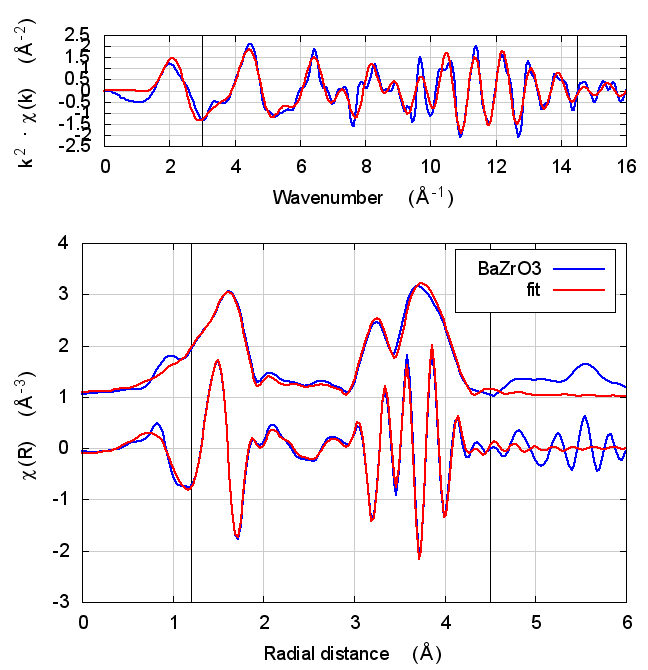
\includegraphics[width=.45\linewidth]{BaZrO3/scf/fit_feff6.png} & 
    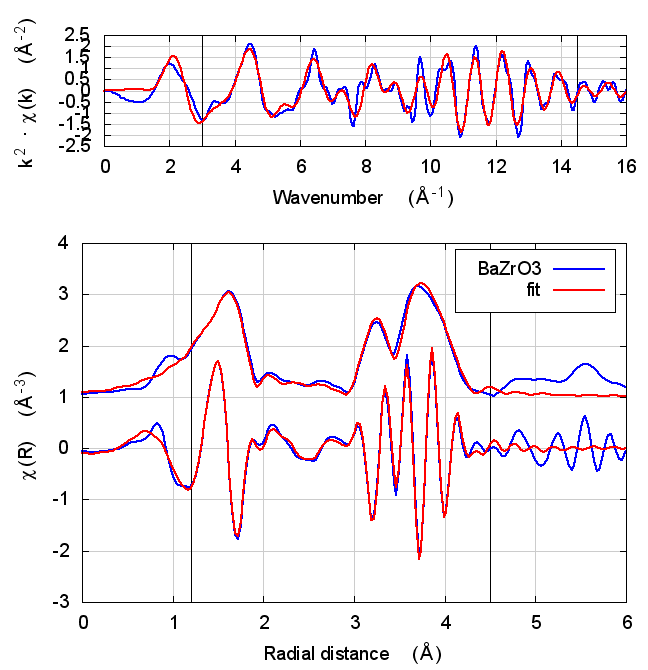
\includegraphics[width=.45\linewidth]{BaZrO3/scf/fit_noSCF.png} \\ 
  \end{tabular}
\end{center}
\begin{center}
  \begin{tabular}{cc}
    \textbf{SCP, R=3} & \textbf{SCP, R=4} \\ 
    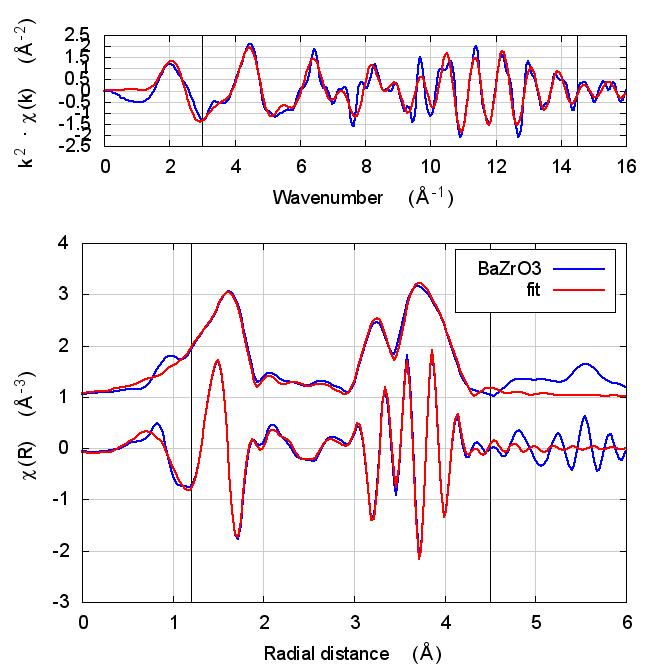
\includegraphics[width=.45\linewidth]{BaZrO3/scf/fit_withSCF_3.png} & 
    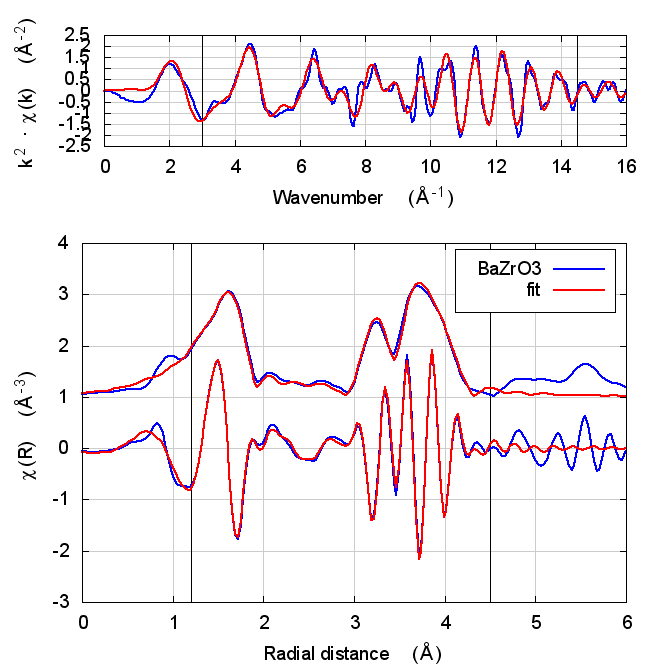
\includegraphics[width=.45\linewidth]{BaZrO3/scf/fit_withSCF_4.png} \\
  \end{tabular}
\end{center}
\begin{center}
  \begin{tabular}{cc}
    \textbf{SCP, R=5} & \textbf{SCP, R=5.5} \\ 
    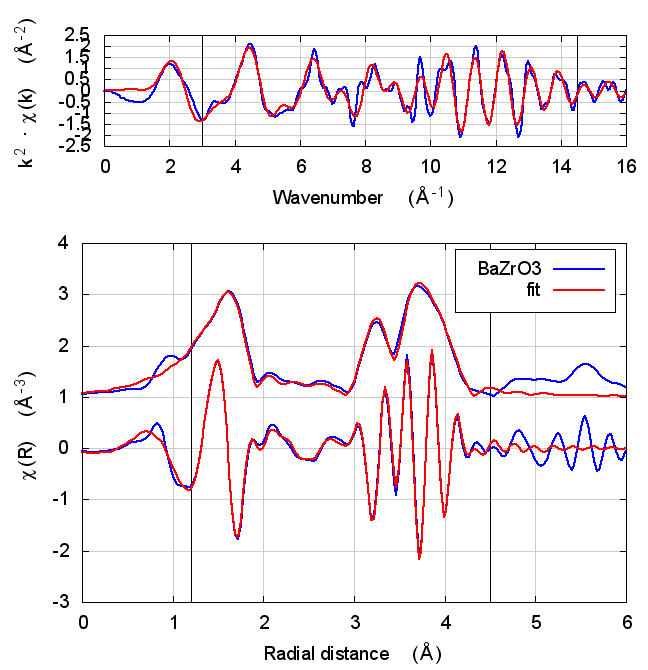
\includegraphics[width=.45\linewidth]{BaZrO3/scf/fit_withSCF_5.png} & 
    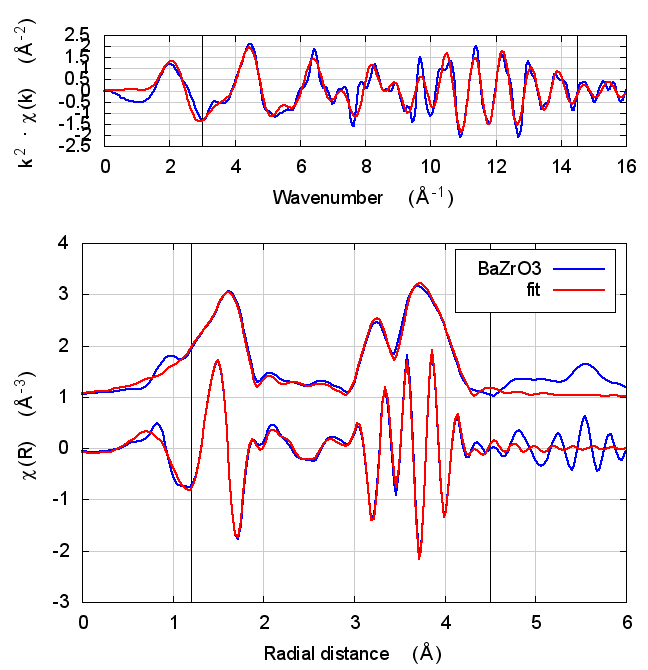
\includegraphics[width=.45\linewidth]{BaZrO3/scf/fit_withSCF_5.5.png} \\
  \end{tabular}
\end{center}
\begin{center}
  \begin{tabular}{cc}
    \textbf{SCP, R=6}&\\
    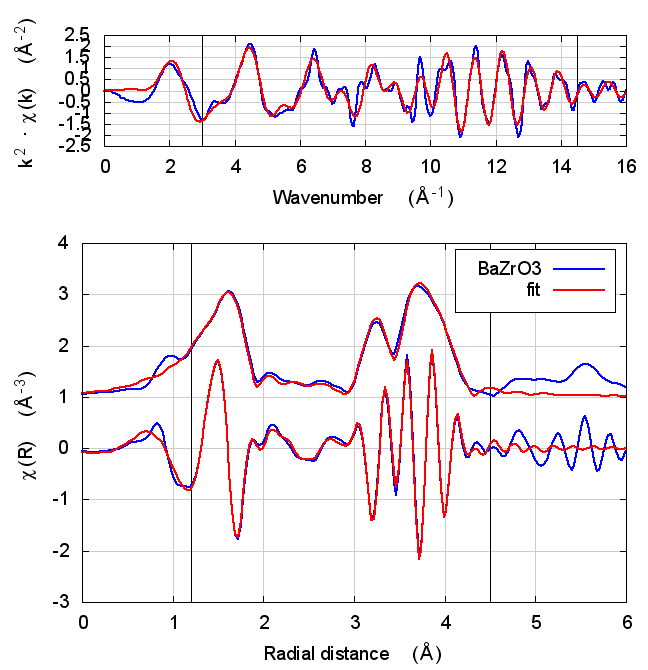
\includegraphics[width=.45\linewidth]{BaZrO3/scf/fit_withSCF_6.png}&\\
  \end{tabular}
\end{center}

\subsection{Discussion}
\label{sec:orgheadline30}

In the paper cited above, the authors speculate that inaccuracies in
Feff's potential model can be accommodated by allowing separate $E_0$
parameters to float for each kind of scatterer. In the paper, the claim
is that the $\Delta$R parameters used to model low temperature BaZrO3 data
correctly follow the trends seen in high temperature XRD data on the
same material.

I didn't quite use the same fitting model as in that paper. Instead of a
variety of $\Delta$R parameters, I used a single isotropic expansion
coefficient, $\alpha$. With just one data set, the fit using many $\Delta$R parameters
was not stable.

The hope, in this case, is that self-consistency and charge transfer
would make all the $E_0$ parameters close to 0 \textbf{and} remove the need for
multiple $E_0$ parameters in the fit. Neither of those hopes were realized.
The $E_0$ parameters in the self-consistent fits were not much different
from the results of the \textsc{feff6} fit and none of them ended up near 0.

Other fitting parameters were, as in other materials, consistent within
uncertainties. In this case, the reduced $\chi^2$ and R-factor were a bit
lower with self-consistency with relative reductions on the same scale
as the increases in FeS2 and NiO.

%\rule{\linewidth}{0.5pt}
%\pagebreak

\section{Bromoadamantane}
\label{sec:orgheadline37}


\begin{wrapfigure}{r}{0.3\textwidth}
  \begin{center}
    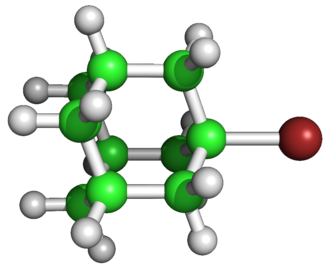
\includegraphics[width=0.3\textwidth]{bromoadamantane/bromoadamantane.png}
  \end{center}
  \caption{1-bromoada-mantane}
\end{wrapfigure}

The data are 1-bromoadamantane. Bromoadamantane is a cycloalkane,
meaning that it is a hydrocarbon with rings of carbon atoms. It is
also a diamondoid, meaning that it is a strong, stiff, 3D network of
covalent bonds. 1-bromoadamantane has one hydrogen atom replaced by a
bromine atom.

The material was supplied by my colleague Dr.\ Alessandra Leri of
Manhattan Marymount College in the form of a white powder. This powder
was spread onto Kapton tape which was folded to make a sample with an
edge step of about 1.7. The data were measured at NSLS beamline X23A2.

This is an interesting test case because it is a molecule (thus the
entire molecule can be included in the self-consistency calculation)
and because there is measurable scattering from the neighboring
hydrogen atoms. While the $\sigma^2$ of the hydrogen scatterers is not
well-determined, the fit is statistically significantly worse when the
hydrogen scatterers are excluded.

The fit includes the nearest neighbor C, the next three C atoms, and
the neighboring 6 hydrogen atoms. The DS triangle paths involving the
first and second neighbor C atoms are also included. The fitting model
assumes that the adamantane anion is very rigid compared to the Br-C
bond. Thus, the formula explained in
\href{http://dx.doi.org/10.1088/1742-6596/190/1/012026}{DOI:
  10.1088/1742-6596/190/1/012026} is used to constrain the second
neighbor C distance to the first neighbor C $\Delta$R parameter.

\begin{figure}[h]
  \centering
  \includegraphics[width=.65\linewidth]{1-bromoadamantane.pdf}
  \caption{$\mu(E)$ data for 1-bromoadamantane, showing the background
    removal spline and the normalization polynomials.}
  \label{fig:bromoadamantane-data}
\end{figure}


\subsection{Best fit values}
\label{sec:orgheadline32}

\begin{center}
  \begin{tabular}{lrrrrrr}
    model & amp & delr & drh & enot & ss & ssh\\
    \hline
    feff6      & 1.57(24) & 0.018(15) & 0.041(20) &  5.95(1.81) & 0.00659(183) & 0.00159(266)\\
    noSCP      & 1.24(22) & 0.017(16) & 0.079(24) & 12.03(1.69) & 0.00554(206) & 0.00008(310)\\
    withSCP(8) & 1.33(20) & 0.018(14) & 0.073(25) &  1.54(1.56) & 0.00560(180) & 0.00143(319)\\
  \end{tabular}
\end{center}

\subsection{Statistical parameters}
\label{sec:orgheadline33}

\begin{center}
  \begin{tabular}{lrrr}
    model & $\chi^2$ & reduced $\chi^2$ & R-factor\\
    \hline
    feff6      &  7744 & 1493 & 0.0207\\
    noSCP      & 10541 & 2033 & 0.0281\\
    withSCP(8) &  8632 & 1665 & 0.0230\\
  \end{tabular}
\end{center}

% \subsection{Charge transfer and threshold energy}
% \label{sec:orgheadline34}

% \begin{center}
% \begin{tabular}{rr}
% ip & R=8\\
% \hline
% 0 & 0.468\\
% 1 & 0.024\\
% 2 & -0.047\\
% $\mu$ & -6.087\\
% \end{tabular}
% \end{center}

% Starting value for $\mu$ in \textsc{feff8} = 4.480

% Value for $\mu$ in \textsc{feff6} = -2.673

\subsection{Plots of fits}
\label{sec:orgheadline35}

\begin{center}
  \begin{tabular}{cc}
    \textbf{Feff6} & \textbf{Feff8, no SCP} \\ 
    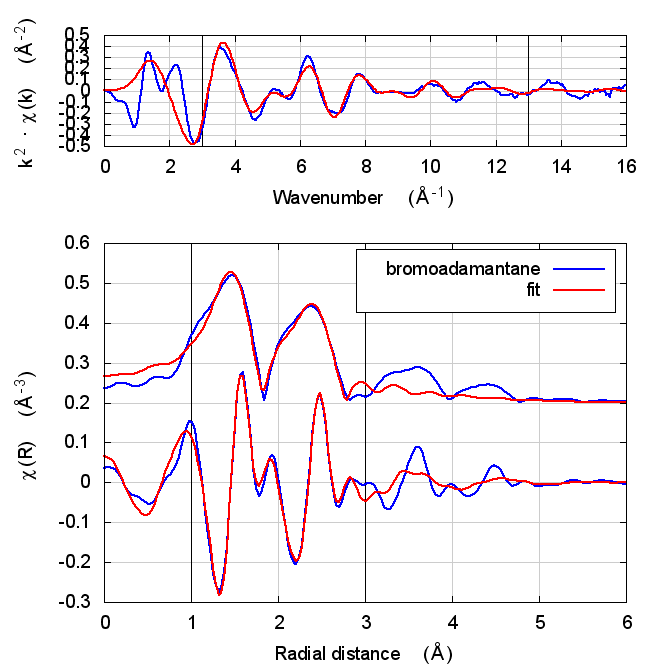
\includegraphics[width=.45\linewidth]{bromoadamantane/scf/fit_feff6.png} & 
    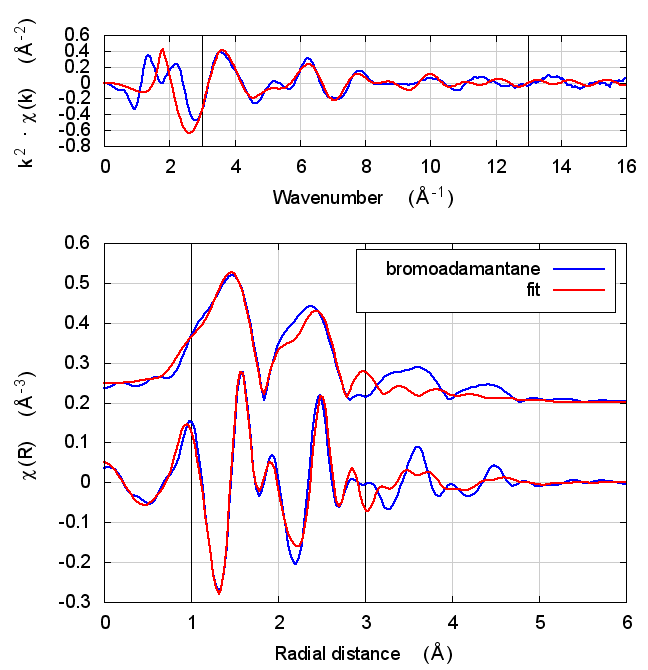
\includegraphics[width=.45\linewidth]{bromoadamantane/scf/fit_noSCF.png} \\
  \end{tabular}
\end{center}
\begin{center}
  \begin{tabular}{cc}
    \textbf{SCP, R=8}&\\
    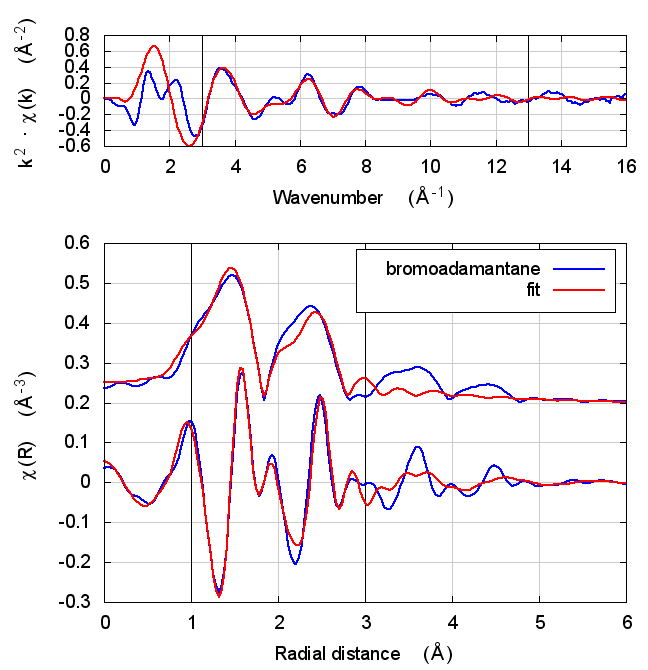
\includegraphics[width=.45\linewidth]{bromoadamantane/scf/fit_withSCF_8.png}&\\
  \end{tabular}
\end{center}

\subsection{Discussion}
\label{sec:orgheadline36}

In June 2015, the
\href{http://www.mail-archive.com/ifeffit@millenia.cars.aps.anl.gov/msg05040.html}{following
  quote} appeared on the
\href{http://cars9.uchicago.edu/mailman/listinfo/ifeffit/}{\textsc{ifeffit}
  mailing list}:

\begin{verbatim}
There are some demonstrated cases where Feff8 is slightly
better than Feff6 at modeling EXAFS. The most notable cases
are when H is in the input file -- Feff6 is terrible at this.
\end{verbatim}

Bromoadamantane is a case where scattering from H atoms can be seen in
the EXAFS data. The statistical parameters are all much smaller when
the H SS path is included in the fit compared to fits which exclude
that scattering path. This is true even though the $\sigma^2$ value
for the H SS path is ill-determined -- its uncertainty is such that
$\sigma^2$ for H is not positive-definite. This is likely because the
small mass of the H atom makes its partial pair distribution function
highly non-Gaussian. The approximation of a simple $\sigma^2$ to model
this distribution is not all that good. Despite the ill-defined
$\sigma^2$, the $\Delta$R is well defined.

The parameters of the first shell C scatterer are quite well defined and
consistent across theory models. $S_0^2$ varies a bit outside of its
uncertainty, as does $\Delta$R for the H atom. The statistical parameters for
the fits with self-consistency and \textsc{feff6} are basically
indistinguishable.

The fitting model is clearly inadequate in the region from 2 {\AA} to
2.5 {\AA}.  The likely cause of this is the fairly rigid constrain
placed on the parameters of the second shell C scatterer. This fitting
model should be re-examined by relaxing this constraint. Future work!

So, is \textsc{feff6} ``terrible'' at handling H scatterers? The
answer may be ``yes'' and may be ``no'', but these data on
bromoadamantane don't suggest that it is any worse than
\textsc{feff8}.

%\rule{\linewidth}{0.5pt}

\section{Uranyl hydrate}
\label{sec:orgheadline43}

\begin{wrapfigure}{r}{0.3\textwidth}
  \begin{center}
    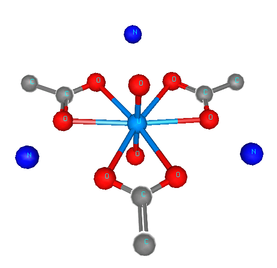
\includegraphics[width=0.3\textwidth]{uranyl/uranyl.png}
  \end{center}
  \caption{The uranyl motif from sodium uranyl triacetate}
\end{wrapfigure}

The data are the hydrated uranyl hydrate shown in Shelly's paper on
\emph{X-ray absorption fine structure determination of pH-dependent
  U-bacterial cell wall interactions},
\href{http://dx.doi.org/10.1016/S0016-7037(02)00947-X}{DOI:
  10.1016/S0016-7037(02)00947-X}

This is an interesting test case because it involves very short
$\sim$1.78{\AA} oxygenyl bonds in an f-electron system.

The \texttt{AFOLP} card was used to run \textsc{feff6}. The
\texttt{FOLP} card with a value of 0.9 for each potential was used to
get \textsc{feff8.5} to run to completion.

Following the lead of that paper, \textsc{feff} was run on the crystal sodium
uranyl triacetate. The relevant bit of the structure is shown in the
figure. For the fitting model, scattering paths related to the axial
and equatorial O atoms (red balls) are used in the fit. Other paths
are unused. The parameterization given in Tables 2 and 5 is used in
this fit.

There is an $S_0^2$ (\texttt{amp}) and an energy shift
(\texttt{enot}). The axial and equatorial oxygen atoms each get a
$\Delta$R (\texttt{deloax} and \texttt{deloeq}) and a $\sigma^2$
(\texttt{sigoax} and \texttt{sigoeq}).

\texttt{amp} is unitless. \texttt{enot} is eV. \texttt{deloax} and
\texttt{deloeq} are {\AA}. \texttt{sigoax} and \texttt{sigoeq} are
{\AA}$^2$.

\begin{figure}[h]
  \centering
  \includegraphics[width=.65\linewidth]{uranyl.pdf}
  \caption{$\mu(E)$ data for uranyl hydrate, showing the background
    removal spline and the normalization polynomials.}
  \label{fig:uranyl-data}
\end{figure}


\subsection{Best fit values}
\label{sec:orgheadline38}

\begin{center}
  \footnotesize
  \begin{tabular}{lrrrrrr}
    model & amp & deloax & deloeq & enot & sigoax & sigoeq\\
    \hline
    feff6        & 0.93(4) & 0.035(40) & -0.043(7)  & 10.63(60) & -0.00007(53) & 0.00726(94)\\
    noSCP        & 1.04(6) & 0.037(52) & -0.054(10) & 11.32(78) &  0.00032(72) & 0.00699(118)\\
    withSCP(2.5) & 1.08(6) & 0.042(55) & -0.045(10) &  3.45(81) &  0.00074(73) & 0.00692(115)\\
    withSCP(2.9) & 1.08(6) & 0.042(55) & -0.045(10) &  3.50(81) &  0.00074(73) & 0.00691(115)\\
    withSCP(4.0) & 1.08(6) & 0.041(55) & -0.045(10) &  3.59(81) &  0.00075(73) & 0.00694(115)\\
    withSCP(5.2) & 1.08(6) & 0.042(55) & -0.045(10) &  3.66(81) &  0.00074(72) & 0.00693(114)\\
    withSCP(6.8) & 1.08(6) & 0.042(55) & -0.045(10) &  3.63(81) &  0.00074(72) & 0.00693(114)\\
  \end{tabular}
\end{center}

\subsection{Statistical parameters}
\label{sec:orgheadline39}

\begin{center}
  \begin{tabular}{lrrr}
    model & $\chi^2$ & reduced $\chi^2$ & R-factor\\
    \hline
    feff6        & 37.7 &  6.1 & 0.0027\\
    noSCP        & 69.1 & 11.1 & 0.0049\\
    withSCP(2.5) & 71.0 & 11.4 & 0.0050\\
    withSCP(2.9) & 70.9 & 11.4 & 0.0050\\
    withSCP(4.0) & 70.4 & 11.3 & 0.0050\\
    withSCP(5.2) & 70.2 & 11.3 & 0.0050\\
    withSCP(6.8) & 70.4 & 11.3 & 0.0050\\
  \end{tabular}
\end{center}

% \subsection{Charge transfer and threshold energy}
% \label{sec:orgheadline40}

% \begin{center}
% \begin{tabular}{rrrrrr}
% ip & R=2.5 & R=2.9 & R=4.0 & R=5.2 & R=6.8\\
% \hline
% 0 & 1.496 & 1.487 & 1.464 & 1.474 & 1.467\\
% 1 & -0.590 & -0.582 & -0.620 & -0.639 & -0.633\\
% 2 & -1.585 & -1.600 & -1.527 & -1.542 & -1.546\\
% 3 & -0.325 & -0.329 & -0.292 & -0.303 & -0.310\\
% 4 & -0.160 & -0.154 & -0.173 & -0.168 & -0.168\\
% 5 & 0.628 & 0.625 & 0.626 & 0.630 & 0.632\\
% $\mu$ & -2.810 & -2.751 & -2.629 & -2.569 & -2.587\\
% \end{tabular}
% \end{center}

% Starting value for $\mu$ in \textsc{feff8} = 6.030

% Value for $\mu$ in \textsc{feff6} = -1.961

\subsection{Plots of fits}
\label{sec:orgheadline41}

\begin{center}
  \begin{tabular}{cc}
    \textbf{Feff6} & \textbf{Feff8, no SCP} \\ 
    \includegraphics[width=.45\linewidth]{uranyl/scf/fit_feff6.png} &
    \includegraphics[width=.45\linewidth]{uranyl/scf/fit_noSCF.png} \\
  \end{tabular}
\end{center}
\begin{center}
  \begin{tabular}{cc}
    \textbf{SCP, R=2.5} & \textbf{SCP, R=2.9} \\ 
    \includegraphics[width=.45\linewidth]{uranyl/scf/fit_withSCF_2.5.png} & 
    \includegraphics[width=.45\linewidth]{uranyl/scf/fit_withSCF_2.9.png} \\
  \end{tabular}
\end{center}
\begin{center}
  \begin{tabular}{cc}
    \textbf{SCP, R=4} & \textbf{SCP, R=5.2} \\ 
    \includegraphics[width=.45\linewidth]{uranyl/scf/fit_withSCF_4.0.png} &
    \includegraphics[width=.45\linewidth]{uranyl/scf/fit_withSCF_5.2.png} \\ 
  \end{tabular}
\end{center}
\begin{center}
  \begin{tabular}{cc}
    \textbf{SCP, R=6.8}&\\
    \includegraphics[width=.45\linewidth]{uranyl/scf/fit_withSCF_6.8.png}&\\
  \end{tabular}
\end{center}

\subsection{Discussion}
\label{sec:orgheadline42}

The most interesting part of this fit is the extremely short, double
bonded, axial oxygen scattering path. With such an extremely rigid bond,
$\sigma^2$ is hard to determine. Even the most sensible result in the table
above gives an answer that is barely positive-definite.

Beyond that parameter, the story here is, by now, familiar. Most fitting
parameters are consistent over the theory models. This is one of the
cases where the statistical parameters are slightly better for \textsc{feff6}
than for any of the \textsc{feff8} fits.

Like with UO2, the $E_0$ values of the self-consistent fits are what one
hopes to find. They are much closer to zero when the edge energy of the
data is chosen at the inflection point of the rising edge. Is this a
trend suggesting that self-consistency is important for setting the
energy scale of f-electron systems?

Also like the UO2 example, the $S_0^2$ value is a bit different using
\textsc{feff6} and \textsc{feff8}, which could have an impact on the interpretation of
the data. It is, however, correlated with the axial $\sigma^2$ result.

%\rule{\linewidth}{0.5pt}

\section{Conclusion}
\label{sec:orgheadline47}

Sometimes (FeS2, uranyl) the statistical parameters suggest the best
fit was found using \textsc{feff6}. Sometimes (BaZrO3) \textsc{feff8}
with self-consistency gave the smaller reduced $\chi^2$ and
R-factor. And sometimes (UO2) it made no difference.

Excepting $E_0$ parameters, the fits presented here yielded equivalent
values for fitting parameters using \textsc{feff6} and \textsc{feff8}
with self-consistency. Only in the case of f-electron systems -- UO2
and uranyl -- were the fitting results for $E_0$ parameters more sensible
with \textsc{feff8} and self-consistency.

In most cases, the fit using \textsc{feff8} without self-consistency
resulted in the largest statistical parameters.

\href{http://bruceravel.github.io/demeter/}{\textsc{artemis}} has used
\textsc{feff6} for years. Nothing presented here suggests that was a
bad idea.

% In the future,
% \href{http://bruceravel.github.io/demeter/}{\textsc{artemis}} will
% likely use
% \href{https://github.com/xraypy/feff85exafs}{\textsc{feff85exafs}}. It
% seems that the most sensible default behavior for
% \href{http://bruceravel.github.io/demeter/}{\textsc{artemis}} would be
% to run
% \href{https://github.com/xraypy/feff85exafs}{\textsc{feff85exafs} } using
% a very short self-consistency radius.

% Is a reviewer justified in demanding that an author use a more recent
% version of \textsc{feff} than \textsc{feff6}? On the basis of what I
% have presented here, I think not.

% \subsection{Theoretical approximations and measurement uncertainty}
% \label{sec:orgheadline44}

% The most valuable result of this effort -- beyond the immediate question
% of the impact of self-consistent potentials on EXAFS analysis -- is that
% these results provide a sense of what level of uncertainty is introduced
% to the application of Gaussian statistics to EXAFS analysis by
% uncertainties in the theory model used as the basis of the fitting.

% \href{http://dx.doi.org/10.1107/S0909049512039544}{This paper}
% attempts to quantify many of the sources of uncertainty in an EXAFS
% measurement. The sort of comparison presented here offers hope of
% quantifying the contribution to the uncertainty budget of the
% measurement due to the approximations that enter into the theory.

\subsection{Interpreting the energy shift parameter}
\label{sec:orgheadline45}

Way back in the early 1990s, in the days of
\href{http://dx.doi.org/10.1103/PhysRevB.44.4146}{\textsc{feff3}}, the
theory was already good enough to get calculated, relative peak
positions very consistent with experimental data in the EXAFS
region. That is, the phase part of the calculation was already highly
reliable for large photoelectron kinetic energies in the very earliest
days of XAS theory.

Consider \href{http://dx.doi.org/10.1103/PhysRevB.83.115106}{this
  paper} on the Bethe-Salpeter equation of motion of the electron-hole
pair.  This is an impressive and successful approach to core-shell
theory, however the positions of peaks in the density of states near
the edge, both above and below, are clearly off.  Consider the MgO
calculation in Fig. 5 of that paper.  It's a great result, but the
peaks are demonstrably shifted relative to experiment.

In the context of finding the threshold energy and the zero of
photoelectron wavenumber, a misplacement of peaks in the DOS will
result in a misplacement of the threshold.  From the \textsc{feff3}
results, we know that an $E_0$ shift is adequate to position the high
kinetic energy peaks well with respect to the data.  Given the
shortcomings even of the current most advanced theory with respect to
finding the absolute energy threshold, it is clear that a parameter
for an overall $E_0$ shift remains necessary to line up the EXAFS data
with the EXAFS theory.  While one must remain mindful that fitted $E_0$
shifts \textbf{can} be
\href{http://dx.doi.org/10.1107/S0909049598002970}{too large}, thus
confounding the measurement of other parameters, EXAFS analysis
continues to require $E_0$ shift parameters.

\end{document}